\documentclass[a4paper]{article}

\usepackage[margin=1in]{geometry} 
\usepackage{amsmath,amsthm,amssymb}
\usepackage{float}
\usepackage{graphicx}
\usepackage[table,xcdraw]{xcolor}
\usepackage[UKenglish]{isodate}
\origdate
\cleanlookdateon
\usepackage[utf8]{inputenc}
\usepackage[hidelinks]{hyperref}
\usepackage{tikz-cd}
\usepackage{enumitem}
\usepackage{mathtools}
% \usepackage{pgfplots}
\usepackage{float}
\usepackage{tikz, venndiagram}
% \usepackage{tkz-euclide}
% \usepackage{tabu}
% \usepackage{framed}
% \usepackage{steinmetz}
\renewcommand{\baselinestretch}{1.5} 
\usepackage[varg]{txfonts}
\usepackage{microtype}
% \usepackage{mathrsfs} 
\usepackage{makecell}
\usepackage{tocloft}
\addtolength{\cftsubsecnumwidth}{10pt}
\usepackage[normalem]{ulem}
\useunder{\uline}{\ul}{}
\usepackage{multirow}
\setcounter{tocdepth}{4}
\setcounter{secnumdepth}{4}
\usepackage{tabularx}

\newcommand*\circled[1]{\tikz[baseline=(char.base)]{
            \node[shape=circle,draw,inner sep=2pt] (char) {#1};}}

% \pgfplotsset{compat=1.16}
\begin{document}
\title{Revision Guide\\[0.1cm]
    \large 30.110 Digital Systems Lab, Term 6 2020}
\author{Wei Min Cher}
\date{23 Oct 2020}

\maketitle

\tableofcontents

\newpage
\section{W1: Introduction}

\subsection{Analog vs Digital Signals}
\begin{table}[H]
\centering
\begin{tabular}{ll}
\multicolumn{1}{c}{{\ul \textbf{Analog signals}}} & \multicolumn{1}{c}{{\ul \textbf{Digital signals}}} \\
- Primitives from physical & - Primitives are Boolean functions \\
- Noise from thermal fluctuations & - Noise from roundoff errors \\
- Error accumulates & - Error does not accumulate through stages
\end{tabular}
\end{table}

\subsection{Fixed-length Encodings}
\begin{itemize}
    \item To represent information in binary, we use fixed-length encodings
    \item e.g. 4-bit binary coded decimal (BCD)
    \begin{itemize}[label=$\circ$]
        \item Total of 10 decimal digits represented by 4 bits\quad $\log_2(10) = 3.322 < 4\text{ bits}$
        \item 10 decimal digits: 0, 1, 2, 3, 4, 5, 6, 7, 8, 9
    \end{itemize}
    \item 7-bit ASCII (American Standard Code for Information Interchange)
    \begin{itemize}[label=$\circ$]
        \item Total of 86 characters represented by 7 bits\quad $\log_2(86) = 6.426 < 7\text{ bits}$
        \item A-Z (26 chars), a-z (26 chars), 0-9 (10 chars), punctuation (11 chars), math (9 chars), financial (4 chars)
    \end{itemize}
\end{itemize}

\subsection{Base Conversion}
\begin{itemize}
    \item Decimal numbers are written normally or with subscript $_{10}$
    \item Octal numbers are prefixed with the letter \textcolor{red}{O} or with subscript $_8$
    \item Hexadecimal numbers are prefixed with \textcolor{red}{0x} or with subscript $_{16}$ 
\end{itemize}

\subsubsection{Converting to Decimal}
$$\text{Total Decimal Value} = \sum_{i=\text{p}_{min}}^{\text{p}_{max}}d_i\cdot(\text{radix})^i$$
\begin{itemize}
    \item In some cases, level of accuracy is specified to reduce number of fractional digits
\end{itemize}

\subsubsection{Converting from Decimal}
\begin{enumerate}
    \item Whole number portion
    \begin{itemize}[label=$\circ$]
        \item Divide decimal number by base of system
        \item Remainder recorded as least significant numeral
        \item Process repeated until quotient of 0 is achieved
    \end{itemize} 
    \newpage
    \item Fractional number portion
    \begin{itemize}[label=$\circ$]
        \item Multiply fractional component by base of system
        \item Whole number recorded as most significant numeral
        \item Process repeated until fractional component equal to zero
    \end{itemize}
    \item Rounding
    \begin{itemize}[label=$\circ$]
        \item Binary: If next bit is $1_2$, round the LSB up. 
        \item Octal: If next bit is $4_8$ or greater, round up.
        \item Hexadecimal: if next bit is $8_{16}$ or greater, round up.
    \end{itemize}
\end{enumerate}


\begin{table}[H]
\centering
\begin{tabular}{c|c|c|c}
\textbf{Decimal} & \textbf{Binary} & \textbf{Octal} & \textbf{Hex} \\ \hline
00 & 0000 & 00 & 0\\
01 & 0001 & 01 & 1 \\
02               & 0010            & 02             & 2            \\
03               & 0011            & 03             & 3            \\ \hline
04               & 0100            & 04             & 4            \\
05               & 0101            & 05             & 5            \\
06               & 0110            & 06             & 6            \\
07               & 0111            & 07             & 7            \\ \hline
08               & 1000            & 10             & 8            \\
09               & 1001            & 11             & 9            \\
10               & 1010            & 12             & A            \\
11               & 1011            & 13             & B            \\ \hline
12               & 1100            & 14             & C            \\
13               & 1101            & 15             & D            \\
14               & 1110            & 16             & E            \\
15               & 1111            & 17             & F           
\end{tabular}
\caption{Number system equivalency}
\end{table}

\subsubsection{Converting between \texorpdfstring{$2^n$}{2n} Bases}

\paragraph{Binary to Octal}
\begin{enumerate}
    \item Form groups of 3 bit representing octal symbols.\quad 
    $(\textcolor{red}{0}10)(111).(01\textcolor{red}{0})_2$
    \item Perform a direct substitution of the bit groupings with the equivalent octal symbol.
    $$(\textcolor{red}{0}10)(111).(01\textcolor{red}{0})_2 = 27.2_8$$
\end{enumerate}

\paragraph{Binary to Hexadecimal}
\begin{enumerate}
    \item Form groups of 4 bit representing hexadecimal symbols. \quad $(\textcolor{red}{00}11)(1011).(1111)(1\textcolor{red}{000})_2$
    \item Perform a direct substitution of the bit groupings with the equivalent hexadecimal symbol.
    $$(\textcolor{red}{00}11)(1011).(1111)(1\textcolor{red}{000})_2 = 3\text{B.F}8_{16}$$
\end{enumerate}

\paragraph{Octal to Binary}
\begin{enumerate}
    \item Each of the octal symbols is replaced with its 3 bit binary equivalent.
    $$347.12_8 = (\textcolor{red}{0}11)(100)(111).(001)(01\textcolor{red}{0})_2 = 11100111.00101_2$$
\end{enumerate}

\paragraph{Hexadecimal to Binary}
\begin{enumerate}
    \item Each of the hexadecimal symbols is replaced with its 4 bit binary equivalent.
    $$1\text{B.A}_{16} = (\textcolor{red}{000}1)(1011).(101\textcolor{red}{0})_2 = 11011.101_2$$
\end{enumerate}

\paragraph{Octal to Hexadecimal}
\begin{enumerate}
    \item Convert the octal number into binary.\quad $71.5_8 = (111)(001).(101)_2 = 111001.101_2$
    \item Convert the binary number into hexadecimal. \quad $(\textcolor{red}{00}11)(1001).(101\textcolor{red}{0})_2 = 39.A_{16}$
\end{enumerate}

\paragraph{Hexadecimal to Octal}
\begin{enumerate}
    \item Convert the hexadecimal number into binary.\quad $\text{AB.C}_{16} = (1010)(1011).(1100)_2 = 10101011.11_2$
    \item Convert the binary number into octal.\quad $(\textcolor{red}{0}10)(101)(011).(11\textcolor{red}{0})_2 = 253.6_8$
\end{enumerate}

\subsection{Two's Complement}
\begin{table}[H]
\centering
\begin{tabular}{cc}
\textbf{Decimal} & \textbf{4-bit Two's Complement} \\ \hline
-8               & \textbf{1}000                   \\
-7               & \textbf{1}001                   \\
-6               & \textbf{1}010                   \\
-5               & \textbf{1}011                   \\ \hline
-4               & \textbf{1}100                   \\
-3               & \textbf{1}101                   \\
-2               & \textbf{1}110                   \\
-1               & \textbf{1}111                   \\ \hline
0                & \textbf{0}000                   \\
1                & \textbf{0}001                   \\
2                & \textbf{0}010                   \\
3                & \textbf{0}011                   \\ \hline
4                & \textbf{0}100                   \\
5                & \textbf{0}101                   \\
6                & \textbf{0}110                   \\
7                & \textbf{0}111                  
\end{tabular}
\end{table}
\begin{itemize}
    \item Range of a $n$-bit two's complement number, $N_\text{2's comp}$: $-(2^{n-1})\leq N_\text{2's comp}\leq 2^{n-1}-1$
    \item Convert two's complement number into decimal number:
    \begin{enumerate}
        \item Sign bit represents -($2^{n-1}$).
        \item Apply $\displaystyle\sum_{i=\text{p}_{min}}^{\text{p}_{max}}d_i\cdot(\text{radix})^i$ to find the corresponding decimal number.
    \end{enumerate}
    \item Taking the two's complement of a number:
    \begin{enumerate}
        \item Perform complement on binary number.
        \item Add 1, ignore carry out if any.
    \end{enumerate}
\end{itemize}

\newpage
\subsubsection{Immunity Representation}
\begin{itemize}
    \item Analogy: strict at sender, tolerant at receiver
    \bigskip
    \begin{figure}[H]
    \centering
    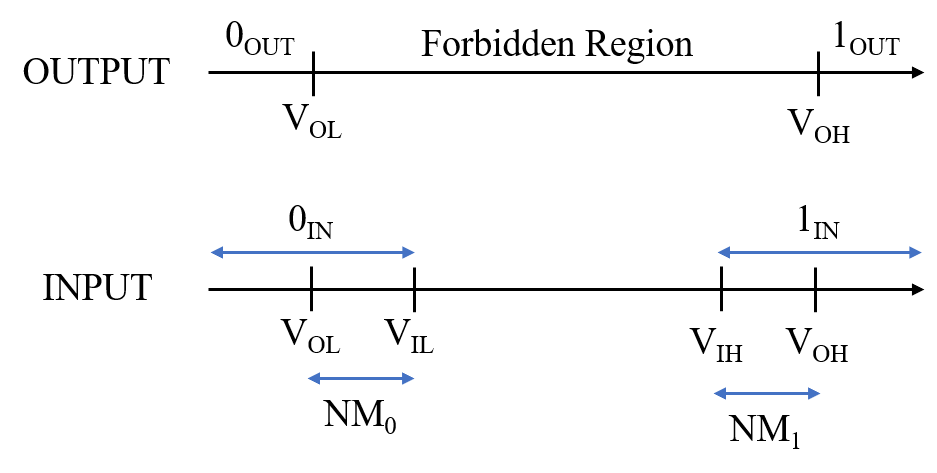
\includegraphics[width=0.5\textwidth]{static-discipline.png}
    \end{figure}
    \item Sending logical 0 ($0_\text{OUT}$): sender produces output voltage $\leq V_{OL}$
    \item Receiving logical 0 ($0_\text{IN}$): receiver receives input voltage $\leq V_{IL}$
    \item Sending logical 1 ($1_\text{OUT}$): sender produces output voltage $\geq V_{OH}$
    \item Receiving logical 1 ($1_\text{IN}$): receiver receives input voltage $\geq V_{IH}$
    \bigskip
    \item Noise margin: absolute value of difference between input and output voltages for given logic value
    $$\text{NM}_{0} = V_{IL} - V_{OL}\qquad \text{NM}_{1} = V_{OH}-V_{IH}$$
    \begin{itemize}[label=$\circ$]
        \item For reasonable noise margin, $V_{OL}\leq V_{IL},\ V_{OH}\geq V_{IH}$.
        \item When $\text{NM}_0 = \text{NM}_1$, noise margins are symmetric.
    \end{itemize}
    \bigskip
    \item Forbidden region: range of voltage levels at which the logic value is undefined
\end{itemize}

\subsection{Timing Specifications}
\begin{itemize}
    \item Propagation delay ($t_\text{PD}$): upper bound on delay from valid inputs to valid outputs
    \begin{itemize}[label=$\circ$] 
        \item Maximum cumulative delay over all paths from inputs to outputs
        \item Design goal: minimize this
        \item Also known as $t_\text{PD,MAX}$
    \end{itemize}
    \item Contamination delay ($t_\text{CD}$): lower bound delay from invalid inputs to invalid outputs
    \begin{itemize}[label=$\circ$]
        \item Minimum cumulative delay over all paths from inputs to outputs
        \item If not specified, can be assumed to be 0.
        \item Important when designing circuits with registers.
        \item Also known as $t_\text{PD,MIN}$
    \end{itemize}
\end{itemize}

\subsection{Combination vs Sequential Logic}
\begin{table}[H]
\centering
\begin{tabular}{ll}
\multicolumn{1}{c}{{\ul \textbf{Combinational logic}}} & \multicolumn{1}{c}{{\ul \textbf{Sequential logic}}} \\
- e.g. calendar, 7-segment LED & - e.g. lock, ATM, traffic light \\
- No state & - State \\
- No memory & - Memory \\
- Truth table & - State diagram
\end{tabular}
\end{table}

\newpage
\section{W2: Boolean Algebra}
\subsection{Basic Definitions}
\begin{itemize}
    \item Set of elements, $S$: collection of objects with common property
    \item Elements, e.g. $x,\ y\in S$: objects that are in the set of elements
    \item Binary operator, e.g. $*,\ +$: rule that assigns to each pair of elements from $S$ a unique element from $S$
\end{itemize}

\subsection{Postulates of Algebraic Systems}
\begin{enumerate}
    \item Closure: A set is closed with respect to a binary operator if it describes a rule for obtaining a unique element of $S$ for every pair of elements in $S$.
    \item Associative law: A binary operator * on set $S$ is associative if $$(x*y)*z = x*(y*z)\text{ for all }x,\ y,\ z \in S.$$
    \item Commutative law: A binary operator * on set $S$ is commutative if $$x*y = y*x\text{ for all }x,\ y \in S.$$
    \item Identity element: A set $S$ has an identity element $e$ with respect to a binary operation * if $$e*x = x*e = x\text{ for every }x\in S.$$
    \item Inverse: A set $S$ with an identity element $e$ has an inverse $y$ when $$x*y = e\text{ every }x\in S.$$
    \item Distributive law: If * and $\cdot$ are two binary operators on the set $S$, * is distributive over $\cdot$ if $$x*(y\cdot z) = (x*y)\cdot(x*z).$$
\end{enumerate}

\subsection{Huntington Postulates}
\begin{enumerate}
    \item Closure:
    \begin{enumerate}[label=\alph*)]
        \item Structure is closed with respect to operator +.
        \item Structure is closed with respect to operator $\cdot$.
    \end{enumerate}
    \item Identity element:
    \begin{enumerate}[label=\alph*)]
        \item 0 is the identity element with respect to +.
        \item 1 is the identity element with respect to $\cdot$.
    \end{enumerate}
    \newpage
    \item Commutative law:
    \begin{enumerate}[label=\alph*)]
        \item Structure is commutative with respect to +.
        \item Structure is commutative with respect to $\cdot$.
    \end{enumerate}
    \item Distributive law:
    \begin{enumerate}[label=\alph*)]
        \item Operator $\cdot$ is distributive over +. \qquad $x\cdot(y+z) = (x\cdot y)+(x\cdot z)$
        \item Operator + is distributive over $\cdot$. \qquad $x+(y\cdot z) = (x+y)\cdot(x+z)$
    \end{enumerate}
    \item For every $x\in B$, there exists a complement $x'\in B$ such that
    \begin{enumerate}
        \item $x+x'=1,$ and
        \item $x\cdot x'=0$.
    \end{enumerate}
    \item There are 2 elements $x,\ y\in B$ such that $x\neq y$.
\end{enumerate}

\subsection{Boolean Algebra vs Ordinary Algebra}
\begin{table}[H]
\centering
\begin{tabular}{l|c|c|}
\cline{2-3}
 & \textbf{Boolean Algebra} & \textbf{Ordinary Algebra} \\ \hline
\multicolumn{1}{|l|}{Associative law} & $\checkmark$ & $\checkmark$ \\ \hline
\multicolumn{1}{|l|}{\begin{tabular}[c]{@{}l@{}}Distributive law of + over $\cdot$\\ $x+(y\cdot z) = (x+y)\cdot(x+z)$\end{tabular}} & $\checkmark$ & $\times$ \\ \hline
\multicolumn{1}{|l|}{Additive or multiplicative inverses} & \begin{tabular}[c]{@{}c@{}}$\times$\\ (No subtraction or division)\end{tabular} & \begin{tabular}[c]{@{}c@{}}$\checkmark$\\ (Subtraction and division)\end{tabular} \\ \hline
\multicolumn{1}{|l|}{Complement} & $\checkmark$ & $\times$ \\ \hline
\multicolumn{1}{|l|}{Elements} & 0, 1 & Real numbers \\ \hline
\end{tabular}
\end{table}

\subsection{Two-Valued Boolean Algebra}
\begin{itemize}
    \item A set of two elements: 0 and 1
    \item Two binary operators equivalent to AND and OR operators
    \item Complement operator equivalent to NOT operator
\end{itemize}

\newpage
\subsection{Basic Theorems and Properties}
\begin{itemize}
    \item Duality
    \begin{itemize}[label=$\circ$]
        \item Every Boolean expression remains valid if the operators and identity elements are interchanged.
    \end{itemize}
    \item Basic Theorems
    \begin{table}[H]
    \centering
    \begin{tabular}{l|c|c|}
    \cline{2-3}
     & \textbf{a)} & \textbf{b)} \\ \hline
    \multicolumn{1}{|l|}{Postulate 2, identity element} & $x + 0 = x$ & $x\cdot 1 = x$ \\ \hline
    \multicolumn{1}{|l|}{Postulate 5, complement} & $x+x' = 1$ & $x\cdot x' = 0$ \\ \hline
    \multicolumn{1}{|l|}{Theorem 1} & $x + x = x$ & $x\cdot x = x$ \\ \hline
    \multicolumn{1}{|l|}{Theorem 2} & $x + 1 = 1$ & $x\cdot 0 = 0$ \\ \hline
    \multicolumn{1}{|l|}{Theorem 3, involution} & \multicolumn{2}{c|}{$(x')' = x$} \\ \hline
    \multicolumn{1}{|l|}{Postulate 3, commutative} & $x + y = y + x$ & $xy = yx$ \\ \hline
    \multicolumn{1}{|l|}{Theorem 4, associative} & $x + (y + z) = (x + y) + z$ & $x(yz) = (xy)z$ \\ \hline
    \multicolumn{1}{|l|}{Postulate 4, distributive} & $x(y + z) = xy + xz$ & $x + yz = (x + y)(x + z)$ \\ \hline
    \multicolumn{1}{|l|}{Theorem 5, De Morgan's Law} & $(x + y)' = x'y'$ & $(xy)' = x' + y'$ \\ \hline
    \multicolumn{1}{|l|}{Theorem 6, absorption} & $x + xy = x$ & $x(x +y) = x$ \\ \hline
    \end{tabular}
    \end{table}
    \begin{itemize}[label=$\circ$]
        \item To prove these theorems, either make use of the postulates or complete the truth table.
        \begin{itemize}[label=\tiny$\blacksquare$]
        \item e.g. Theorems 1b and 2b are dual of theorems 1a and 2a. 
        \item Each step of proof in Theorems 1b and 2b is the dual of its counterpart in Theorems 1a and 2a.
    \end{itemize}
    \end{itemize}
    \item By manipulating the Boolean expression, it is possible to obtain a simpler expression.
\end{itemize}

\newpage
\subsection{Minterms and Maxterms}
\begin{itemize}
    \item Minterms: logical AND of a set of variables
    \begin{itemize}[label=$\circ$]
        \item Primed if 0, unprimed if 1
    \end{itemize}
    \item Maxterms: logical OR of a set of variables
    \begin{itemize}[label=$\circ$]
        \item Primed if 1, unprimed if 0
    \end{itemize}
\begin{table}[H]
\centering
\begin{tabular}{ccccccc}
 &  &  & \multicolumn{2}{c}{\textbf{Minterms}} & \multicolumn{2}{c}{\textbf{Maxterms}} \\
x & y & z & Term & Designation & Term & Designation \\
\hline
0 & 0 & 0 & $x'y'z'$ & $m_0$ & $x + y + z$ & $M_0$ \\
0 & 0 & 1 & $x'y'z$ & $m_1$ & $x + y + z'$ & $M_1$ \\
0 & 1 & 0 & $x'yz'$ & $m_2$ & $x + y' + z$ & $M_2$ \\
0 & 1 & 1 & $x'yz$ & $m_3$ & $x + y' + z'$ & $M_3$ \\
1 & 0 & 0 & $xy'z'$ & $m_4$ & $x' + y + z$ & $M_4$ \\
1 & 0 & 1 & $xy'z$ & $m_5$ & $x' + y + z'$ & $M_5$ \\
1 & 1 & 0 & $xyz'$ & $m_6$ & $x' + y' + z$ & $M_6$ \\
1 & 1 & 1 & $xyz$ & $m_7$ & $x' + y' + z'$ & $M_7$
\end{tabular}
\end{table}
\item Any Boolean function can be expressed algebraically by taking sum of minterms which produce a 1.
\item Any Boolean function can be expressed algebraically by taking product of maxterms which produce a 0.
\end{itemize}

\subsection{Conversion between Minterms and Maxterms}
\begin{itemize}
    \item Complement of sum of minterms = Sum of minterms missing in original function
    \begin{itemize}[label=$\circ$]
        \item e.g. F(A, B, C) = $\sum(1, 4, 7) = m_1+m_4+m_7$\\
        $\Rightarrow$ F'(A, B, C) = $\sum(0, 2, 3, 5, 6) = m_0+m_2+m_3+m_5+m_6$
    \end{itemize}
    \item Using De Morgan's Theorem on F', we can express F as a product of maxterms:
    \begin{align*}
        \text{F(A, B, C) = (F'(A, B, C))'} &= (m_0+m_2+m_3+m_5+m_6)'\\
        &= m_0'm_2'm_3'm_5'm_6'\\
        &= M_0M_2M_3M_5M_6 = \Pi(0, 2, 3, 5, 6)
    \end{align*}
    \item Maxterm $M_i$ is complement of minterm $m_i$. \qquad $m_i' = M_i$
\end{itemize}

\subsection{Two and Three-Level Implementation}
\begin{itemize}
    \item Two-level implementation preferred: produces least amount of delay
    \item However, number of inputs to logic gates may not practical.
    \item In those cases, one could use a three-level implementation instead.
\end{itemize}

\subsection{Digital Logic Gates}
\begin{figure}[H]
    \centering
    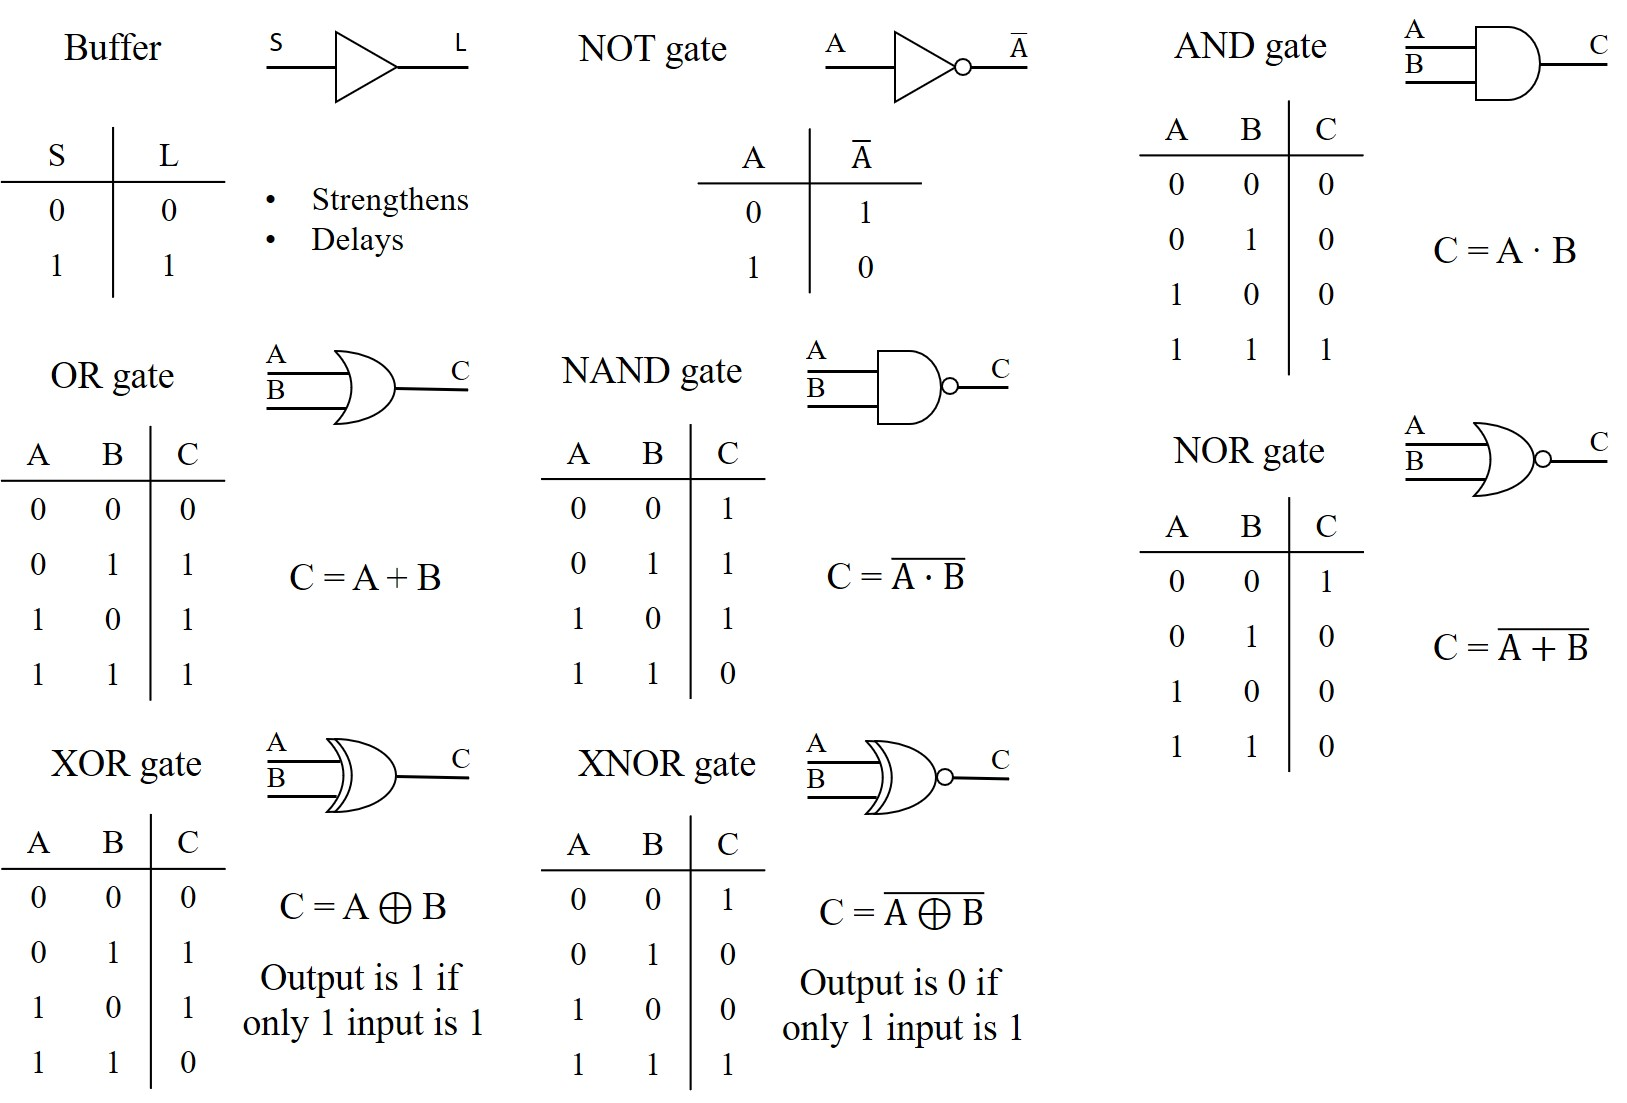
\includegraphics[width=\textwidth]{logicgates.jpg}
\end{figure}

\subsection{Signal Logic and Logic Polarity}
\begin{itemize}
    \item Positive logic system: choosing logical high to represent logic 1
    \item Negative logic system: choosing logical low to represent logic 1
    \item Wedges are added at inputs and outputs to signify a negative logic gate.
\end{itemize}
\newpage
\section{W2: Gate-Level Minimization}

\subsection{K-Map}
\begin{center}
\begin{minipage}[c]{0.2\textwidth}
\begin{table}[H]
\centering
\begin{tabular}{ccc}
 & 0 & 1 \\ \cline{2-3} 
\multicolumn{1}{c|}{0} & \multicolumn{1}{c|}{$m_0$} & \multicolumn{1}{c|}{$m_1$} \\ \cline{2-3} 
\multicolumn{1}{c|}{1} & \multicolumn{1}{c|}{$m_2$} & \multicolumn{1}{c|}{$m_3$} \\ \cline{2-3} 
\end{tabular}
\end{table}
\end{minipage}
\begin{minipage}[c]{0.35\textwidth}
\begin{table}[H]
\centering
\begin{tabular}{ccccc}
 & 00 & 01 & 11 & 10 \\ \cline{2-5} 
\multicolumn{1}{c|}{0} & \multicolumn{1}{c|}{$m_0$} & \multicolumn{1}{c|}{$m_1$} & \multicolumn{1}{c|}{$m_3$} & \multicolumn{1}{c|}{$m_2$} \\ \cline{2-5} 
\multicolumn{1}{c|}{1} & \multicolumn{1}{c|}{$m_4$} & \multicolumn{1}{c|}{$m_5$} & \multicolumn{1}{c|}{$m_7$} & \multicolumn{1}{c|}{$m_6$} \\ \cline{2-5} 
\end{tabular}
\end{table}
\end{minipage}
\begin{minipage}[c]{0.3\textwidth}
\begin{table}[H]
\centering
\begin{tabular}{ccccc}
 & 00 & 01 & 11 & 10 \\ \cline{2-5} 
\multicolumn{1}{c|}{00} & \multicolumn{1}{c|}{$m_0$} & \multicolumn{1}{c|}{$m_1$} & \multicolumn{1}{c|}{$m_3$} & \multicolumn{1}{c|}{$m_2$} \\ \cline{2-5} 
\multicolumn{1}{c|}{01} & \multicolumn{1}{c|}{$m_4$} & \multicolumn{1}{c|}{$m_5$} & \multicolumn{1}{c|}{$m_7$} & \multicolumn{1}{c|}{$m_6$} \\ \cline{2-5} 
\multicolumn{1}{c|}{11} & \multicolumn{1}{c|}{$m_{12}$} & \multicolumn{1}{c|}{$m_{13}$} & \multicolumn{1}{c|}{$m_{15}$} & \multicolumn{1}{c|}{$m_{14}$} \\ \cline{2-5} 
\multicolumn{1}{c|}{10} & \multicolumn{1}{c|}{$m_8$} & \multicolumn{1}{c|}{$m_9$} & \multicolumn{1}{c|}{$m_{11}$} & \multicolumn{1}{c|}{$m_{10}$} \\ \cline{2-5} 
\end{tabular}
\end{table}
\end{minipage}
\end{center}

\subsubsection{General Rules}
\begin{itemize}
    \item Priority should go to drawing the largest squares possible, grouping either 2, 4 or 8 minterms together.
    \item The larger the squares, the simpler the expression.
    \item All minterms with 1's should be covered when we combine squares.
\end{itemize}

\subsubsection{Product of Sums Simplification}
\begin{itemize}
    \item Combine squares with 0's, then apply De Morgan's theorem to obtain the product of sums expression.
\end{itemize}

\subsection{Don't Care Conditions}
\begin{itemize}
    \item Function is not specified for some combinations or we don't care
    \item X is used for don't care conditions
    \item Can be assumed to be either 0 or 1
\end{itemize}

\subsection{NAND and NOR Implementation}
\begin{itemize}
    \item Any logic circuit can be implemented using NAND and NOR gates
    \item Using De Morgan's Theorem: \quad $\overline{A\cdot B} = \overline{A}+\overline{B} \qquad \overline{A+B} = \overline{A}\cdot\overline{B}$
\end{itemize}

\newpage
\section{W2: Time Response}

\subsection{Gate Delays}
\begin{itemize}
    \item Signal propagation is not instantaneous
    \item Glitches: unwanted transient output changes
    \begin{itemize}[label=$\circ$]
        \item Occurs when different pathways have different delays
    \end{itemize}
    \item Hazard: logic circuit with potential for glitches
\end{itemize}

\subsection{Types of Hazards}
\begin{itemize}
    \item Static hazards
    \begin{itemize}[label=$\circ$]
        \item Brief glitch to other logic state
    \end{itemize}
    \item Dynamic hazards
    \begin{itemize}[label=$\circ$]
        \item Multiple transitions instead of clean transition
    \end{itemize}
\end{itemize}

\subsection{Eliminating Static Hazards}
\begin{itemize}
    \item Use clock signals
    \item Lengthen waiting interval
    \item Add redundant K-map encirclements
    \begin{itemize}[label=$\circ$]
        \item To eliminate static 1-hazards: use SOP form
        \item To eliminate static 0-hazards: use POS form
        \item Only works for 2-level logic
    \end{itemize}
\end{itemize}

\newpage
\section{W3: Combinational Logic}
\subsection{Combinational Circuit}
\begin{itemize}
    \item Circuit with \textit{n} inputs, \textit{m} outputs
    \item No feedback paths or memory elements
\end{itemize}

\subsection{Design Process}
\begin{enumerate}
    \item Understand the problem.
    \begin{itemize}[label=$\circ$]
        \item e.g. \textit{Build a circuit that converts from binary-coded decimal (BCD) to excess-3 binary code.}
    \end{itemize}
    \item From the circuit specifications, find the required number of inputs and outputs, assigning a symbol to each.
    \begin{itemize}[label=$\circ$]
        \item e.g. \textit{For the circuit, there will be 4 inputs A, B, C and D and 4 outputs w, x, y and z.}
    \end{itemize}
    \item Derive a truth table that defines the required relationship between inputs and outputs.
    \begin{table}[H]
    \centering
    \begin{tabular}{lllllcccc}
     & \multicolumn{4}{c}{\textbf{\begin{tabular}[c]{@{}c@{}}Inputs \\ (BCD)\end{tabular}}} & \multicolumn{4}{c}{\textbf{\begin{tabular}[c]{@{}c@{}}Outputs \\ (Excess-3)\end{tabular}}} \\ \cline{2-9} 
     & \multicolumn{1}{c}{\textbf{A}} & \multicolumn{1}{c}{\textbf{B}} & \multicolumn{1}{c}{\textbf{C}} & \multicolumn{1}{c|}{\textbf{D}} & \textbf{w} & \textbf{x} & \textbf{y} & \textbf{z} \\
     & 0 & 0 & 0 & \multicolumn{1}{l|}{0} & 0 & 0 & 1 & 1 \\
     & 0 & 0 & 0 & \multicolumn{1}{l|}{1} & 0 & 1 & 0 & 0 \\
     & 0 & 0 & 1 & \multicolumn{1}{l|}{0} & 0 & 1 & 0 & 1 \\
     & 0 & 0 & 1 & \multicolumn{1}{l|}{1} & 0 & 1 & 1 & 0 \\
     & 0 & 1 & 0 & \multicolumn{1}{l|}{0} & 0 & 1 & 1 & 1 \\
     & 0 & 1 & 0 & \multicolumn{1}{l|}{1} & 1 & 0 & 0 & 0 \\
     & 0 & 1 & 1 & \multicolumn{1}{l|}{0} & 1 & 0 & 0 & 1 \\
     & 0 & 1 & 1 & \multicolumn{1}{l|}{1} & 1 & 0 & 1 & 0 \\
     & 1 & 0 & 0 & \multicolumn{1}{l|}{0} & 1 & 0 & 1 & 1 \\
     & 1 & 0 & 0 & \multicolumn{1}{l|}{1} & 1 & 1 & 0 & 0 \\ \hline
    \multirow{2}{*}{\begin{tabular}[c]{@{}l@{}}Don't Care\\ Conditions\end{tabular}} & 1 & 0 & 1 & \multicolumn{1}{l|}{0} & x & x & x & x \\
     & 1 & 0 & 1 & \multicolumn{1}{l|}{1} & x & x & x & x \\
     & 1 & 1 & 0 & \multicolumn{1}{l|}{0} & x & x & x & x \\
     & 1 & 1 & 0 & \multicolumn{1}{l|}{1} & x & x & x & x \\
     & 1 & 1 & 1 & \multicolumn{1}{l|}{0} & x & x & x & x \\
     & 1 & 1 & 1 & \multicolumn{1}{l|}{1} & x & x & x & x
    \end{tabular}
    \end{table}
    \newpage
    \item Obtain simplified Boolean functions for each output as a function of input variables using K-maps.\\ \textcolor{red}{\textbf{Check for wrap-arounds!}}
    \begin{figure}[H]
    \centering
    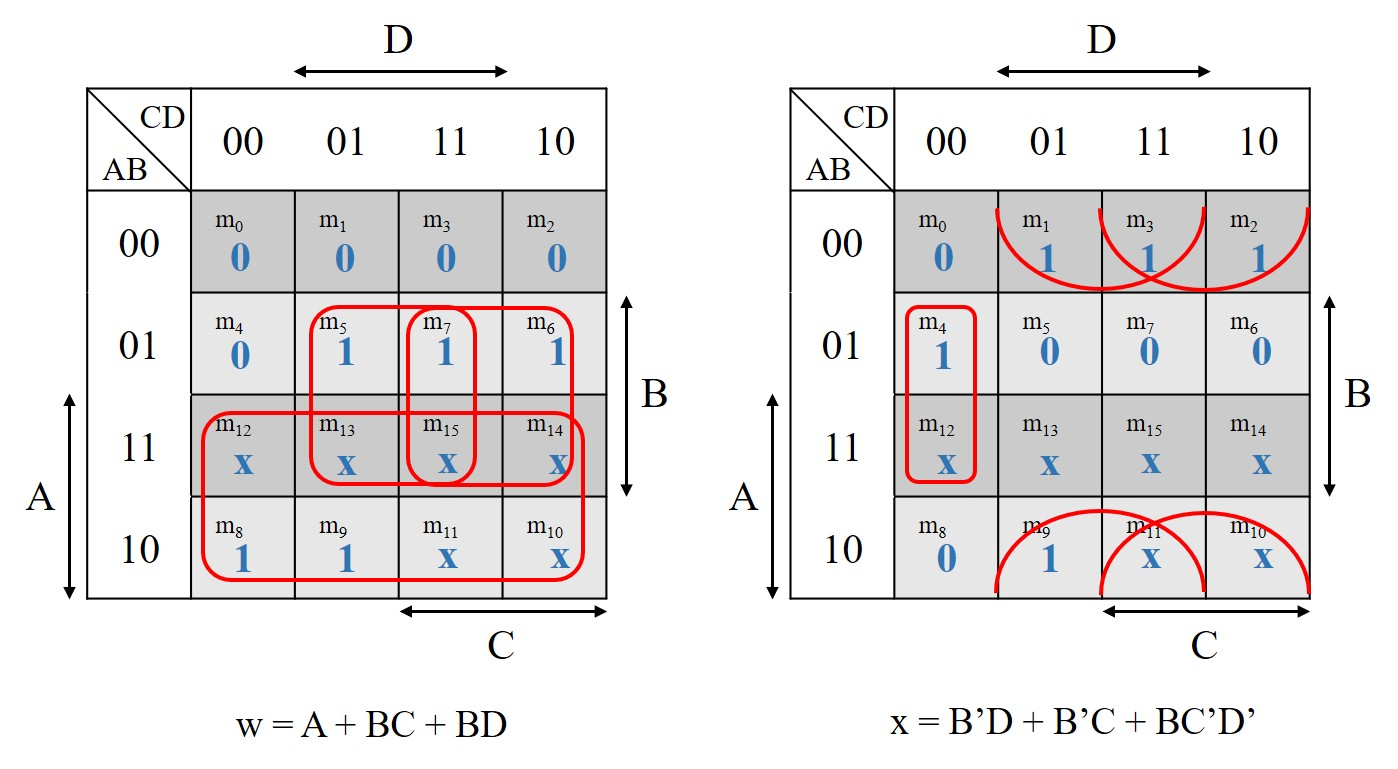
\includegraphics[width=0.75\textwidth]{wx.jpg}\\
    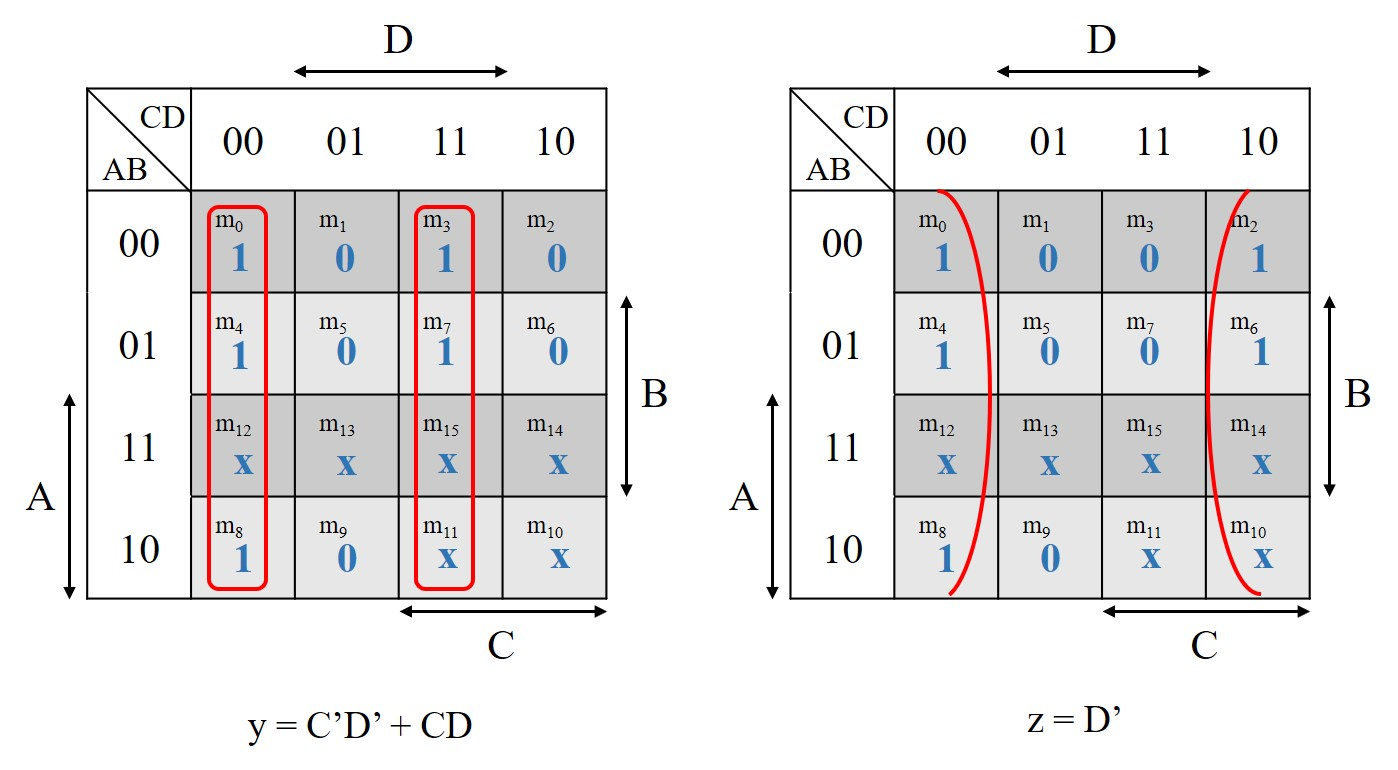
\includegraphics[width=0.75\textwidth]{yz.jpg}
    \end{figure}
    \item Verify the correctness of the design either manually or by simulation.
\end{enumerate}

\newpage
\section{W4: Sequential Circuits}

\subsection{Overview}
\begin{itemize}
    \item Sequential circuit: present output depends on present input(s) and output(s)
    \begin{enumerate}
        \item Synchronous sequential circuit: synchronised by clock signal
        \begin{itemize}[label=$\circ$]
            \item Reacts to changes slower \quad e.g. flip-flops
        \end{itemize}
        \item Asynchronous sequential circuit: not synchronised by clock signal
        \begin{itemize}[label=$\circ$]
            \item Reacts to changes quicker \quad e.g. latches
        \end{itemize}
    \end{enumerate}
    \item Combinational circuit: present output depends on present input(s)
\end{itemize}

\subsection{Latches}
\begin{itemize}
    \item Basic storage element
    \item Stores either 0 or 1.
\end{itemize}

\subsubsection{SR Latch}
\begin{minipage}{0.4\textwidth}
\begin{center}
\tikzset{every picture/.style={line width=0.75pt}}      
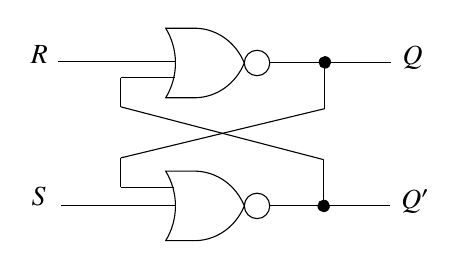
\begin{tikzpicture}[x=0.75pt,y=0.75pt,yscale=-1,xscale=1]
\draw    (203.5,148.21) -- (260,148.21) ;
\draw  [fill={rgb, 255:red, 255; green, 255; blue, 255 }  ,fill opacity=1 ] (293.25,148.71) .. controls (293.25,145.33) and (295.99,142.59) .. (299.38,142.59) .. controls (302.76,142.59) and (305.5,145.33) .. (305.5,148.71) .. controls (305.5,152.1) and (302.76,154.84) .. (299.38,154.84) .. controls (295.99,154.84) and (293.25,152.1) .. (293.25,148.71) -- cycle ;
\draw    (305.5,148.43) -- (364.07,148.43) ;
\draw  [fill={rgb, 255:red, 0; green, 0; blue, 0 }  ,fill opacity=1 ] (329.3,148.43) .. controls (329.3,146.91) and (330.53,145.69) .. (332.04,145.69) .. controls (333.56,145.69) and (334.79,146.91) .. (334.79,148.43) .. controls (334.79,149.94) and (333.56,151.17) .. (332.04,151.17) .. controls (330.53,151.17) and (329.3,149.94) .. (329.3,148.43) -- cycle ;
\draw    (205,217.29) -- (260,217.29) ;
\draw  [fill={rgb, 255:red, 255; green, 255; blue, 255 }  ,fill opacity=1 ] (293.25,217.57) .. controls (293.25,214.19) and (295.99,211.45) .. (299.38,211.45) .. controls (302.76,211.45) and (305.5,214.19) .. (305.5,217.57) .. controls (305.5,220.95) and (302.76,223.7) .. (299.38,223.7) .. controls (295.99,223.7) and (293.25,220.95) .. (293.25,217.57) -- cycle ;
\draw    (304.93,217.57) -- (363.5,217.57) ;
\draw  [fill={rgb, 255:red, 0; green, 0; blue, 0 }  ,fill opacity=1 ] (328.73,217.57) .. controls (328.73,216.06) and (329.96,214.83) .. (331.47,214.83) .. controls (332.99,214.83) and (334.21,216.06) .. (334.21,217.57) .. controls (334.21,219.09) and (332.99,220.31) .. (331.47,220.31) .. controls (329.96,220.31) and (328.73,219.09) .. (328.73,217.57) -- cycle ;
\draw    (332.04,151.17) -- (332.04,170.71) ;
\draw    (233.79,208.57) -- (259.5,208.57) ;
\draw    (233.79,194.43) -- (233.79,208.57) ;
\draw    (332.04,170.71) -- (233.79,194.43) ;
\draw    (233.79,155.71) -- (260,155.71) ;
\draw    (233.79,155.71) -- (233.79,169.86) ;
\draw    (331.47,195.29) -- (331.47,214.83) ;
\draw    (233.79,169.86) -- (331.47,195.29) ;
\draw   (255.39,131.97) -- (269.95,131.97) .. controls (280.11,132.27) and (289.19,138.8) .. (293.25,148.71) .. controls (289.19,158.63) and (280.11,165.15) .. (269.95,165.46) -- (255.39,165.46) .. controls (261.63,155.1) and (261.63,142.33) .. (255.39,131.97) -- cycle;
\draw   (255.39,200.83) -- (269.95,200.83) .. controls (280.11,201.13) and (289.19,207.66) .. (293.25,217.57) .. controls (289.19,227.49) and (280.11,234.01) .. (269.95,234.31) -- (255.39,234.31) .. controls (261.63,223.95) and (261.63,211.19) .. (255.39,200.83) -- cycle;
\draw (367.93,139.26) node [anchor=north west][inner sep=0.75pt]    {$Q$};
\draw (367.36,208.4) node [anchor=north west][inner sep=0.75pt]    {$Q'$};
\draw (189.14,138.97) node [anchor=north west][inner sep=0.75pt]    {$R$};
\draw (189.5,207.19) node [anchor=north west][inner sep=0.75pt]    {$S$};
\end{tikzpicture}
\end{center}
\end{minipage}
\begin{minipage}{0.3\textwidth}
\begin{table}[H]
\centering
\begin{tabular}{cc|cc}
S & R & Q & Q'\\ \hline
0 & 0 & \multicolumn{2}{c}{Memory}\\
0 & 1 & 0 & 1\\
1 & 0 & 1 & 0\\
1 & 1 & \multicolumn{2}{c}{Forbidden}
\end{tabular}
\end{table}
\end{minipage}
\begin{minipage}{0.3\textwidth}
\begin{center}
\tikzset{every picture/.style={line width=0.75pt}}
\begin{tikzpicture}[x=0.75pt,y=0.75pt,yscale=-1,xscale=1]
\draw   (153,71.5) -- (223,71.5) -- (223,177.5) -- (153,177.5) -- cycle ;
\draw    (120.5,100) -- (152.5,100) ;
\draw    (120.5,149.5) -- (152.5,149.5) ;
\draw    (223,99.5) -- (255,99.5) ;
\draw    (223,150) -- (255,150) ;
\draw  [fill={rgb, 255:red, 255; green, 255; blue, 255 }  ,fill opacity=1 ] (223,150) .. controls (223,146.62) and (225.74,143.88) .. (229.13,143.88) .. controls (232.51,143.88) and (235.25,146.62) .. (235.25,150) .. controls (235.25,153.38) and (232.51,156.13) .. (229.13,156.13) .. controls (225.74,156.13) and (223,153.38) .. (223,150) -- cycle ;
\draw (160,91.4) node [anchor=north west][inner sep=0.75pt]    {$S$};
\draw (158,141.4) node [anchor=north west][inner sep=0.75pt]    {$R$};
\end{tikzpicture}
\end{center}
\end{minipage}

\subsubsection{S'R' Latch}
\begin{minipage}{0.4\textwidth}
\begin{center}
\tikzset{every picture/.style={line width=0.75pt}}       
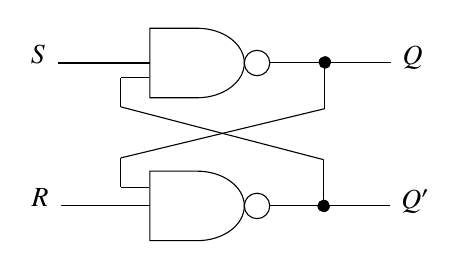
\begin{tikzpicture}[x=0.75pt,y=0.75pt,yscale=-1,xscale=1]
\draw    (203.5,148.71) -- (247.79,148.71) ;
\draw   (247.75,131.96) -- (270.5,131.96) .. controls (283.06,131.96) and (293.25,139.46) .. (293.25,148.71) .. controls (293.25,157.97) and (283.06,165.46) .. (270.5,165.46) -- (247.75,165.46) -- cycle ;
\draw  [fill={rgb, 255:red, 255; green, 255; blue, 255 }  ,fill opacity=1 ] (293.25,148.71) .. controls (293.25,145.33) and (295.99,142.59) .. (299.38,142.59) .. controls (302.76,142.59) and (305.5,145.33) .. (305.5,148.71) .. controls (305.5,152.1) and (302.76,154.84) .. (299.38,154.84) .. controls (295.99,154.84) and (293.25,152.1) .. (293.25,148.71) -- cycle ;
\draw    (305.5,148.43) -- (364.07,148.43) ;
\draw  [fill={rgb, 255:red, 0; green, 0; blue, 0 }  ,fill opacity=1 ] (329.3,148.43) .. controls (329.3,146.91) and (330.53,145.69) .. (332.04,145.69) .. controls (333.56,145.69) and (334.79,146.91) .. (334.79,148.43) .. controls (334.79,149.94) and (333.56,151.17) .. (332.04,151.17) .. controls (330.53,151.17) and (329.3,149.94) .. (329.3,148.43) -- cycle ;
\draw    (205,217.29) -- (247.79,217.29) ;
\draw   (247.75,200.82) -- (270.5,200.82) .. controls (283.06,200.82) and (293.25,208.32) .. (293.25,217.57) .. controls (293.25,226.82) and (283.06,234.32) .. (270.5,234.32) -- (247.75,234.32) -- cycle ;
\draw  [fill={rgb, 255:red, 255; green, 255; blue, 255 }  ,fill opacity=1 ] (293.25,217.57) .. controls (293.25,214.19) and (295.99,211.45) .. (299.38,211.45) .. controls (302.76,211.45) and (305.5,214.19) .. (305.5,217.57) .. controls (305.5,220.95) and (302.76,223.7) .. (299.38,223.7) .. controls (295.99,223.7) and (293.25,220.95) .. (293.25,217.57) -- cycle ;
\draw    (304.93,217.57) -- (363.5,217.57) ;
\draw  [fill={rgb, 255:red, 0; green, 0; blue, 0 }  ,fill opacity=1 ] (328.73,217.57) .. controls (328.73,216.06) and (329.96,214.83) .. (331.47,214.83) .. controls (332.99,214.83) and (334.21,216.06) .. (334.21,217.57) .. controls (334.21,219.09) and (332.99,220.31) .. (331.47,220.31) .. controls (329.96,220.31) and (328.73,219.09) .. (328.73,217.57) -- cycle ;
\draw    (332.04,151.17) -- (332.04,170.71) ;
\draw    (233.79,208.57) -- (247.5,208.57) ;
\draw    (233.79,194.43) -- (233.79,208.57) ;
\draw    (332.04,170.71) -- (233.79,194.43) ;
\draw    (233.79,155.71) -- (247.5,155.71) ;
\draw    (233.79,155.71) -- (233.79,169.86) ;
\draw    (331.47,195.29) -- (331.47,214.83) ;
\draw    (233.79,169.86) -- (331.47,195.29) ;
\draw (367.93,139.26) node [anchor=north west][inner sep=0.75pt]    {$Q$};
\draw (367.36,208.4) node [anchor=north west][inner sep=0.75pt]    {$Q'$};
\draw (189.14,138.97) node [anchor=north west][inner sep=0.75pt]    {$S$};
\draw (189.5,207.69) node [anchor=north west][inner sep=0.75pt]    {$R$};
\end{tikzpicture}
\end{center}
\end{minipage}
\begin{minipage}{0.3\textwidth}
\begin{table}[H]
\centering
\begin{tabular}{cc|cc}
S & R & Q & Q'\\ \hline
0 & 0 & \multicolumn{2}{c}{Forbidden}\\
0 & 1 & 1 & 0\\
1 & 0 & 0 & 1\\
1 & 1 & \multicolumn{2}{c}{Memory}
\end{tabular}
\end{table}
\end{minipage}
\begin{minipage}{0.3\textwidth}
\begin{center}
\tikzset{every picture/.style={line width=0.75pt}}  
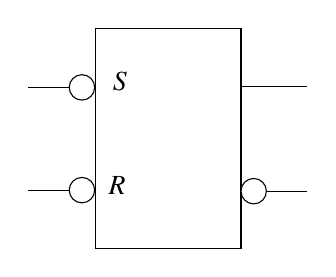
\begin{tikzpicture}[x=0.75pt,y=0.75pt,yscale=-1,xscale=1]
\draw   (153,71.5) -- (223,71.5) -- (223,177.5) -- (153,177.5) -- cycle ;
\draw    (120.5,100) -- (152.5,100) ;
\draw    (120.5,149.5) -- (152.5,149.5) ;
\draw    (223,99.5) -- (255,99.5) ;
\draw    (223,150) -- (255,150) ;
\draw  [fill={rgb, 255:red, 255; green, 255; blue, 255 }  ,fill opacity=1 ] (223,150) .. controls (223,146.62) and (225.74,143.88) .. (229.13,143.88) .. controls (232.51,143.88) and (235.25,146.62) .. (235.25,150) .. controls (235.25,153.38) and (232.51,156.13) .. (229.13,156.13) .. controls (225.74,156.13) and (223,153.38) .. (223,150) -- cycle ;
\draw  [fill={rgb, 255:red, 255; green, 255; blue, 255 }  ,fill opacity=1 ] (140.25,100) .. controls (140.25,96.62) and (142.99,93.88) .. (146.38,93.88) .. controls (149.76,93.88) and (152.5,96.62) .. (152.5,100) .. controls (152.5,103.38) and (149.76,106.13) .. (146.38,106.13) .. controls (142.99,106.13) and (140.25,103.38) .. (140.25,100) -- cycle ;
\draw  [fill={rgb, 255:red, 255; green, 255; blue, 255 }  ,fill opacity=1 ] (140.25,149.5) .. controls (140.25,146.12) and (142.99,143.38) .. (146.38,143.38) .. controls (149.76,143.38) and (152.5,146.12) .. (152.5,149.5) .. controls (152.5,152.88) and (149.76,155.63) .. (146.38,155.63) .. controls (142.99,155.63) and (140.25,152.88) .. (140.25,149.5) -- cycle ;
\draw (160,91.4) node [anchor=north west][inner sep=0.75pt]    {$S$};
\draw (158,141.4) node [anchor=north west][inner sep=0.75pt]    {$R$};
\end{tikzpicture}
\end{center}
\end{minipage}

\newpage
\subsubsection{SR Latch with Control Input}
\begin{minipage}{0.65\textwidth}
\begin{center}
\tikzset{every picture/.style={line width=0.75pt}}   
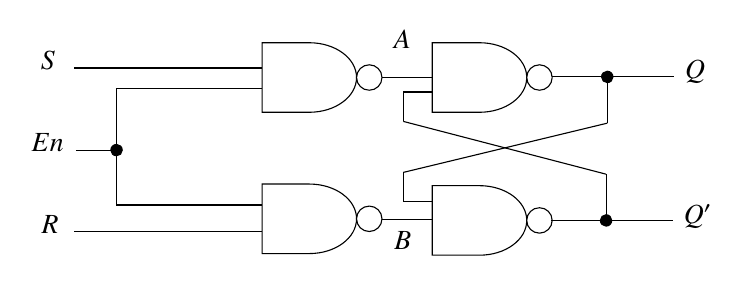
\begin{tikzpicture}[x=0.75pt,y=0.75pt,yscale=-1,xscale=1]
\draw   (189.25,69.96) -- (212,69.96) .. controls (224.56,69.96) and (234.75,77.46) .. (234.75,86.71) .. controls (234.75,95.97) and (224.56,103.46) .. (212,103.46) -- (189.25,103.46) -- cycle ;
\draw  [fill={rgb, 255:red, 255; green, 255; blue, 255 }  ,fill opacity=1 ] (234.75,86.71) .. controls (234.75,83.33) and (237.49,80.59) .. (240.88,80.59) .. controls (244.26,80.59) and (247,83.33) .. (247,86.71) .. controls (247,90.1) and (244.26,92.84) .. (240.88,92.84) .. controls (237.49,92.84) and (234.75,90.1) .. (234.75,86.71) -- cycle ;
\draw   (189.25,138.04) -- (212,138.04) .. controls (224.56,138.04) and (234.75,145.53) .. (234.75,154.79) .. controls (234.75,164.04) and (224.56,171.54) .. (212,171.54) -- (189.25,171.54) -- cycle ;
\draw  [fill={rgb, 255:red, 255; green, 255; blue, 255 }  ,fill opacity=1 ] (234.75,154.79) .. controls (234.75,151.4) and (237.49,148.66) .. (240.88,148.66) .. controls (244.26,148.66) and (247,151.4) .. (247,154.79) .. controls (247,158.17) and (244.26,160.91) .. (240.88,160.91) .. controls (237.49,160.91) and (234.75,158.17) .. (234.75,154.79) -- cycle ;
\draw   (189.25,148.14) -- (119,148.14) -- (119,124.71) ;
\draw   (189.25,92.14) -- (119,92.14) -- (119,119.86) ;
\draw  [fill={rgb, 255:red, 0; green, 0; blue, 0 }  ,fill opacity=1 ] (116.37,121.69) .. controls (116.37,120.17) and (117.6,118.95) .. (119.12,118.95) .. controls (120.63,118.95) and (121.86,120.17) .. (121.86,121.69) .. controls (121.86,123.2) and (120.63,124.43) .. (119.12,124.43) .. controls (117.6,124.43) and (116.37,123.2) .. (116.37,121.69) -- cycle ;
\draw    (98.71,82.14) -- (189.29,82.14) ;
\draw    (98.71,161) -- (189.29,161) ;
\draw    (99.57,121.69) -- (116.37,121.69) ;
\draw    (247,86.71) -- (271.29,86.71) ;
\draw   (271.25,69.96) -- (294,69.96) .. controls (306.56,69.96) and (316.75,77.46) .. (316.75,86.71) .. controls (316.75,95.97) and (306.56,103.46) .. (294,103.46) -- (271.25,103.46) -- cycle ;
\draw  [fill={rgb, 255:red, 255; green, 255; blue, 255 }  ,fill opacity=1 ] (316.75,86.71) .. controls (316.75,83.33) and (319.49,80.59) .. (322.88,80.59) .. controls (326.26,80.59) and (329,83.33) .. (329,86.71) .. controls (329,90.1) and (326.26,92.84) .. (322.88,92.84) .. controls (319.49,92.84) and (316.75,90.1) .. (316.75,86.71) -- cycle ;
\draw    (329,86.43) -- (387.57,86.43) ;
\draw  [fill={rgb, 255:red, 0; green, 0; blue, 0 }  ,fill opacity=1 ] (352.8,86.43) .. controls (352.8,84.91) and (354.03,83.69) .. (355.54,83.69) .. controls (357.06,83.69) and (358.29,84.91) .. (358.29,86.43) .. controls (358.29,87.94) and (357.06,89.17) .. (355.54,89.17) .. controls (354.03,89.17) and (352.8,87.94) .. (352.8,86.43) -- cycle ;
\draw    (247,155.29) -- (271.29,155.29) ;
\draw   (271.25,138.82) -- (294,138.82) .. controls (306.56,138.82) and (316.75,146.32) .. (316.75,155.57) .. controls (316.75,164.82) and (306.56,172.32) .. (294,172.32) -- (271.25,172.32) -- cycle ;
\draw  [fill={rgb, 255:red, 255; green, 255; blue, 255 }  ,fill opacity=1 ] (316.75,155.57) .. controls (316.75,152.19) and (319.49,149.45) .. (322.88,149.45) .. controls (326.26,149.45) and (329,152.19) .. (329,155.57) .. controls (329,158.95) and (326.26,161.7) .. (322.88,161.7) .. controls (319.49,161.7) and (316.75,158.95) .. (316.75,155.57) -- cycle ;
\draw    (328.43,155.57) -- (387,155.57) ;
\draw  [fill={rgb, 255:red, 0; green, 0; blue, 0 }  ,fill opacity=1 ] (352.23,155.57) .. controls (352.23,154.06) and (353.46,152.83) .. (354.97,152.83) .. controls (356.49,152.83) and (357.71,154.06) .. (357.71,155.57) .. controls (357.71,157.09) and (356.49,158.31) .. (354.97,158.31) .. controls (353.46,158.31) and (352.23,157.09) .. (352.23,155.57) -- cycle ;
\draw    (355.54,89.17) -- (355.54,108.71) ;
\draw    (257.29,146.57) -- (271,146.57) ;
\draw    (257.29,132.43) -- (257.29,146.57) ;
\draw    (355.54,108.71) -- (257.29,132.43) ;
\draw    (257.29,93.71) -- (271,93.71) ;
\draw    (257.29,93.71) -- (257.29,107.86) ;
\draw    (354.97,133.29) -- (354.97,152.83) ;
\draw    (257.29,107.86) -- (354.97,133.29) ;
\draw (81.43,72.97) node [anchor=north west][inner sep=0.75pt]    {$S$};
\draw (81.71,151.83) node [anchor=north west][inner sep=0.75pt]    {$R$};
\draw (76.57,112.4) node [anchor=north west][inner sep=0.75pt]    {$En$};
\draw (391.43,77.26) node [anchor=north west][inner sep=0.75pt]    {$Q$};
\draw (390.86,146.4) node [anchor=north west][inner sep=0.75pt]    {$Q'$};
\draw (251.14,62.97) node [anchor=north west][inner sep=0.75pt]    {$A$};
\draw (251.29,159.83) node [anchor=north west][inner sep=0.75pt]    {$B$};
\end{tikzpicture}
\end{center}
\end{minipage}
\begin{minipage}{0.1\textwidth}
\begin{table}[H]
\begin{tabular}{ccc|cc}
En & S & R & Q & Q' \\ \hline
0 & x & x & \multicolumn{2}{c}{Memory} \\
1 & 0 & 0 & \multicolumn{2}{c}{Memory} \\
1 & 0 & 1 & 0 & 1 \\
1 & 1 & 0 & 1 & 0 \\
1 & 1 & 1 & \multicolumn{2}{c}{Forbidden}
\end{tabular}
\end{table}
\end{minipage}
\begin{itemize}
    \item Outputs stay as long as enable signal is 0.
    \item When enable input is 1, info from inputs can affect latch.
\end{itemize}

\subsubsection{D Latch}
\begin{center}
\tikzset{every picture/.style={line width=0.75pt}}      
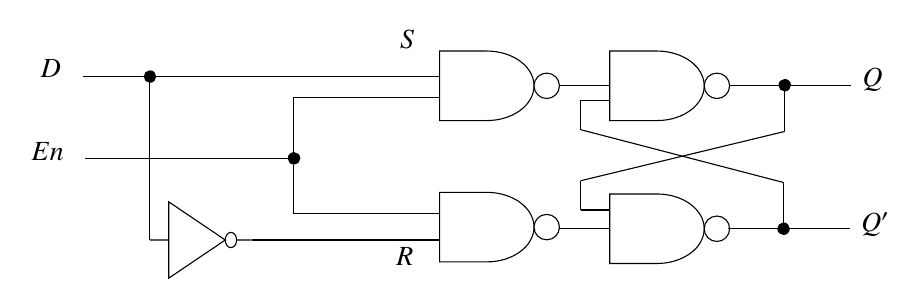
\begin{tikzpicture}[x=0.75pt,y=0.75pt,yscale=-1,xscale=1]
\draw   (312.25,89.96) -- (335,89.96) .. controls (347.56,89.96) and (357.75,97.46) .. (357.75,106.71) .. controls (357.75,115.97) and (347.56,123.46) .. (335,123.46) -- (312.25,123.46) -- cycle ;
\draw  [fill={rgb, 255:red, 255; green, 255; blue, 255 }  ,fill opacity=1 ] (357.75,106.71) .. controls (357.75,103.33) and (360.49,100.59) .. (363.88,100.59) .. controls (367.26,100.59) and (370,103.33) .. (370,106.71) .. controls (370,110.1) and (367.26,112.84) .. (363.88,112.84) .. controls (360.49,112.84) and (357.75,110.1) .. (357.75,106.71) -- cycle ;
\draw   (312.25,158.04) -- (335,158.04) .. controls (347.56,158.04) and (357.75,165.53) .. (357.75,174.79) .. controls (357.75,184.04) and (347.56,191.54) .. (335,191.54) -- (312.25,191.54) -- cycle ;
\draw  [fill={rgb, 255:red, 255; green, 255; blue, 255 }  ,fill opacity=1 ] (357.75,174.79) .. controls (357.75,171.4) and (360.49,168.66) .. (363.88,168.66) .. controls (367.26,168.66) and (370,171.4) .. (370,174.79) .. controls (370,178.17) and (367.26,180.91) .. (363.88,180.91) .. controls (360.49,180.91) and (357.75,178.17) .. (357.75,174.79) -- cycle ;
\draw   (312.25,168.14) -- (242,168.14) -- (242,144.71) ;
\draw   (312.25,112.14) -- (242,112.14) -- (242,139.86) ;
\draw  [fill={rgb, 255:red, 0; green, 0; blue, 0 }  ,fill opacity=1 ] (239.38,141.69) .. controls (239.38,140.17) and (240.6,138.95) .. (242.12,138.95) .. controls (243.63,138.95) and (244.86,140.17) .. (244.86,141.69) .. controls (244.86,143.2) and (243.63,144.43) .. (242.12,144.43) .. controls (240.6,144.43) and (239.38,143.2) .. (239.38,141.69) -- cycle ;
\draw    (140.5,102.14) -- (312.29,102.14) ;
\draw    (221.71,181) -- (312.29,181) ;
\draw    (141.5,141.69) -- (239.38,141.69) ;
\draw    (370,106.71) -- (394.29,106.71) ;
\draw   (394.25,89.96) -- (417,89.96) .. controls (429.56,89.96) and (439.75,97.46) .. (439.75,106.71) .. controls (439.75,115.97) and (429.56,123.46) .. (417,123.46) -- (394.25,123.46) -- cycle ;
\draw  [fill={rgb, 255:red, 255; green, 255; blue, 255 }  ,fill opacity=1 ] (439.75,106.71) .. controls (439.75,103.33) and (442.49,100.59) .. (445.88,100.59) .. controls (449.26,100.59) and (452,103.33) .. (452,106.71) .. controls (452,110.1) and (449.26,112.84) .. (445.88,112.84) .. controls (442.49,112.84) and (439.75,110.1) .. (439.75,106.71) -- cycle ;
\draw    (452,106.43) -- (510.57,106.43) ;
\draw  [fill={rgb, 255:red, 0; green, 0; blue, 0 }  ,fill opacity=1 ] (475.8,106.43) .. controls (475.8,104.91) and (477.03,103.69) .. (478.54,103.69) .. controls (480.06,103.69) and (481.29,104.91) .. (481.29,106.43) .. controls (481.29,107.94) and (480.06,109.17) .. (478.54,109.17) .. controls (477.03,109.17) and (475.8,107.94) .. (475.8,106.43) -- cycle ;
\draw    (370,175.29) -- (394.29,175.29) ;
\draw   (394.25,158.82) -- (417,158.82) .. controls (429.56,158.82) and (439.75,166.32) .. (439.75,175.57) .. controls (439.75,184.82) and (429.56,192.32) .. (417,192.32) -- (394.25,192.32) -- cycle ;
\draw  [fill={rgb, 255:red, 255; green, 255; blue, 255 }  ,fill opacity=1 ] (439.75,175.57) .. controls (439.75,172.19) and (442.49,169.45) .. (445.88,169.45) .. controls (449.26,169.45) and (452,172.19) .. (452,175.57) .. controls (452,178.95) and (449.26,181.7) .. (445.88,181.7) .. controls (442.49,181.7) and (439.75,178.95) .. (439.75,175.57) -- cycle ;
\draw    (451.43,175.57) -- (510,175.57) ;
\draw  [fill={rgb, 255:red, 0; green, 0; blue, 0 }  ,fill opacity=1 ] (475.23,175.57) .. controls (475.23,174.06) and (476.46,172.83) .. (477.97,172.83) .. controls (479.49,172.83) and (480.71,174.06) .. (480.71,175.57) .. controls (480.71,177.09) and (479.49,178.31) .. (477.97,178.31) .. controls (476.46,178.31) and (475.23,177.09) .. (475.23,175.57) -- cycle ;
\draw    (478.54,109.17) -- (478.54,128.71) ;
\draw    (380.29,166.57) -- (394,166.57) ;
\draw    (380.29,152.43) -- (380.29,166.57) ;
\draw    (478.54,128.71) -- (380.29,152.43) ;
\draw    (380.29,113.71) -- (394,113.71) ;
\draw    (380.29,113.71) -- (380.29,127.86) ;
\draw    (477.97,153.29) -- (477.97,172.83) ;
\draw    (380.29,127.86) -- (477.97,153.29) ;
\draw   (181.79,162.63) -- (209.01,181) -- (181.79,199.38) -- (181.79,162.63) -- cycle (172.71,181) -- (181.79,181) (214.46,181) -- (221.71,181) (209.01,181) .. controls (209.01,178.97) and (210.23,177.33) .. (211.73,177.33) .. controls (213.24,177.33) and (214.46,178.97) .. (214.46,181) .. controls (214.46,183.03) and (213.24,184.68) .. (211.73,184.68) .. controls (210.23,184.68) and (209.01,183.03) .. (209.01,181) -- cycle ;
\draw    (172.71,102.25) -- (172.71,181) ;
\draw  [fill={rgb, 255:red, 0; green, 0; blue, 0 }  ,fill opacity=1 ] (169.97,102.25) .. controls (169.97,100.74) and (171.2,99.51) .. (172.71,99.51) .. controls (174.23,99.51) and (175.46,100.74) .. (175.46,102.25) .. controls (175.46,103.76) and (174.23,104.99) .. (172.71,104.99) .. controls (171.2,104.99) and (169.97,103.76) .. (169.97,102.25) -- cycle ;
\draw (291.93,78.97) node [anchor=north west][inner sep=0.75pt]    {$S$};
\draw (290.21,183.33) node [anchor=north west][inner sep=0.75pt]    {$R$};
\draw (114.07,132.9) node [anchor=north west][inner sep=0.75pt]    {$En$};
\draw (514.43,97.26) node [anchor=north west][inner sep=0.75pt]    {$Q$};
\draw (513.86,166.4) node [anchor=north west][inner sep=0.75pt]    {$Q'$};
\draw (118.57,92.9) node [anchor=north west][inner sep=0.75pt]    {$D$};
\end{tikzpicture}
\end{center}
\bigskip

\begin{minipage}{0.6\textwidth}
\begin{table}[H]
\centering
\begin{tabular}{cc|c}
En & D & $Q(t+1)$ \\ \hline
0 & x & $Q(t)$ \\
1 & 0 & 0 \\
1 & 1 & 1
\end{tabular}
\end{table}
\end{minipage}
\begin{minipage}{0.25\textwidth}
\begin{center}
\tikzset{every picture/.style={line width=0.75pt}}
\begin{tikzpicture}[x=0.75pt,y=0.75pt,yscale=-1,xscale=1]
\draw   (153,71.5) -- (223,71.5) -- (223,177.5) -- (153,177.5) -- cycle ;
\draw    (120.5,100) -- (152.5,100) ;
\draw    (120.5,149.5) -- (152.5,149.5) ;
\draw    (223,99.5) -- (255,99.5) ;
\draw    (223,150) -- (255,150) ;
\draw  [fill={rgb, 255:red, 255; green, 255; blue, 255 }  ,fill opacity=1 ] (223,150) .. controls (223,146.62) and (225.74,143.88) .. (229.13,143.88) .. controls (232.51,143.88) and (235.25,146.62) .. (235.25,150) .. controls (235.25,153.38) and (232.51,156.13) .. (229.13,156.13) .. controls (225.74,156.13) and (223,153.38) .. (223,150) -- cycle ;
\draw (160,91.4) node [anchor=north west][inner sep=0.75pt]    {$D$};
\draw (158,141.4) node [anchor=north west][inner sep=0.75pt]    {$En$};
\end{tikzpicture}
\end{center}
\end{minipage}
\begin{itemize}
    \item Eliminates condition when S and R are both 1.
    \item Holds data in internal storage.
    \item Output follows inputs as long as enable input is 1.
\end{itemize}

\subsection{Latch vs Flip-flop}
\begin{itemize}
    \item Latch: operate with signal levels
    \begin{itemize}[label=$\circ$]
        \item e.g. level sensitive devices
    \end{itemize}
    \item Flip-flops: controlled by clock transitions (positive/negative-edge responses)
    \begin{itemize}[label=$\circ$]
        \item e.g. edge sensitive devices
    \end{itemize}
\end{itemize}

\subsection{Flip-flops}
\begin{itemize}
    \item Storage elements that are controlled by clock transitions.
    \item Stores either 0 or 1.
\end{itemize}

\subsubsection{D Flip-flop}
\begin{itemize}
    \item Implementation of D latch using clock transitions instead of level transitions
    \item Value of $D$ transferred to $Q$ upon clock transition
    \item Characteristic equation: $Q(t+1) = D$
\end{itemize}
\begin{table}[H]
\centering
\begin{tabular}{c|l}
D & \multicolumn{1}{c}{$Q(t+1)$} \\ \hline
0 & 0\quad Reset \\
1 & 1\quad Set
\end{tabular}
\end{table}

\paragraph{Negative-edge-triggered}
\begin{itemize}
    \item Also known as master-slave D flip-flop
    \item Value of $D$ transferred to $Q$ upon negative clock transition from 1 to 0
\end{itemize}
\begin{center}
\tikzset{every picture/.style={line width=0.75pt}}    
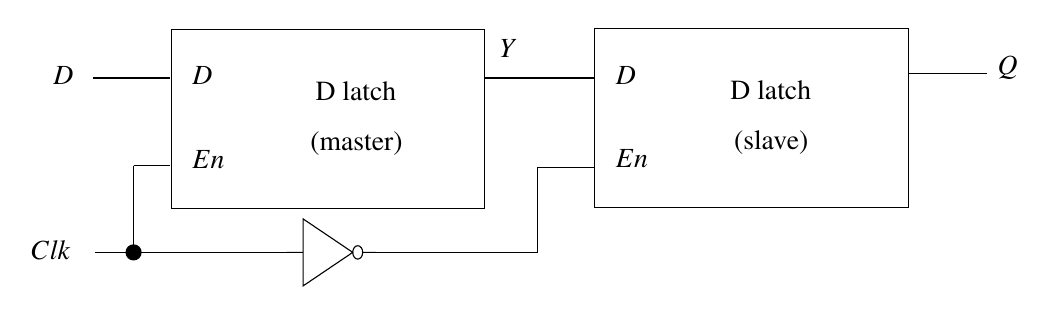
\begin{tikzpicture}[x=0.75pt,y=0.75pt,yscale=-1,xscale=1]
\draw   (168.5,95.5) -- (319.5,95.5) -- (319.5,181.79) -- (168.5,181.79) -- cycle ;
\draw    (130.5,119) -- (168,119) ;
\draw    (131.5,203) -- (224,203) ;
\draw    (150.25,161.25) -- (150.25,203) ;
\draw    (150.25,161.25) -- (168,161.25) ;
\draw  [color={rgb, 255:red, 0; green, 0; blue, 0 }  ,draw opacity=1 ][fill={rgb, 255:red, 0; green, 0; blue, 0 }  ,fill opacity=1 ] (146.63,203) .. controls (146.63,201) and (148.25,199.38) .. (150.25,199.38) .. controls (152.25,199.38) and (153.88,201) .. (153.88,203) .. controls (153.88,205) and (152.25,206.63) .. (150.25,206.63) .. controls (148.25,206.63) and (146.63,205) .. (146.63,203) -- cycle ;
\draw   (231.96,186.88) -- (255.85,203) -- (231.96,219.13) -- (231.96,186.88) -- cycle (224,203) -- (231.96,203) (260.63,203) -- (267,203) (255.85,203) .. controls (255.85,201.22) and (256.92,199.78) .. (258.24,199.78) .. controls (259.56,199.78) and (260.63,201.22) .. (260.63,203) .. controls (260.63,204.78) and (259.56,206.23) .. (258.24,206.23) .. controls (256.92,206.23) and (255.85,204.78) .. (255.85,203) -- cycle ;
\draw   (372.5,95) -- (523.5,95) -- (523.5,181.29) -- (372.5,181.29) -- cycle ;
\draw    (319.5,119) -- (372.5,119) ;
\draw    (524,117) -- (561.5,117) ;
\draw    (267,203) -- (345,203) ;
\draw   (345,203) -- (345,162.25) -- (372,162.25) ;
\draw (177,112) node [anchor=north west][inner sep=0.75pt]    {$D$};
\draw (177,152.4) node [anchor=north west][inner sep=0.75pt]    {$En$};
\draw (229,119.5) node [anchor=north west][inner sep=0.75pt]   [align=left] {\begin{minipage}[lt]{40.693784pt}\setlength\topsep{0pt}
\begin{center}
D latch\\(master)
\end{center}
\end{minipage}};
\draw (110,112) node [anchor=north west][inner sep=0.75pt]    {$D$};
\draw (99.5,196) node [anchor=north west][inner sep=0.75pt]    {$Clk$};
\draw (381,112) node [anchor=north west][inner sep=0.75pt]    {$D$};
\draw (381,151.9) node [anchor=north west][inner sep=0.75pt]    {$En$};
\draw (433,119) node [anchor=north west][inner sep=0.75pt]   [align=left] {\begin{minipage}[lt]{34.4675pt}\setlength\topsep{0pt}
\begin{center}
D latch\\(slave)
\end{center}
\end{minipage}};
\draw (325,98.9) node [anchor=north west][inner sep=0.75pt]    {$Y$};
\draw (565,107.4) node [anchor=north west][inner sep=0.75pt]    {$Q$};
\end{tikzpicture}
\end{center}
\begin{minipage}{0.6\textwidth}
\begin{center}
\begin{table}[H]
\centering
\begin{tabular}{cc|cc}
Clk & D & Q & Q' \\ \hline
$\downarrow$ & 0 & 0 & 1 \\
$\downarrow$ & 1 & 1 & 0
\end{tabular}
\end{table}
\end{center}
\end{minipage}
\begin{minipage}{0.3\textwidth}
\begin{center}
\tikzset{every picture/.style={line width=0.75pt}}       
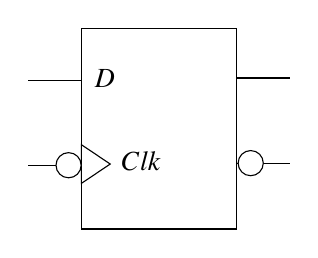
\begin{tikzpicture}[x=0.75pt,y=0.75pt,yscale=-1,xscale=1]
\draw   (167,71.5) -- (242,71.5) -- (242,168.25) -- (167,168.25) -- cycle ;
\draw   (181,136.93) -- (167.13,146.25) -- (167.13,127.62) -- cycle ;
\draw    (141.5,96.5) -- (167,96.5) ;
\draw    (141.5,137.5) -- (167,137.5) ;
\draw    (242,95.5) -- (267.5,95.5) ;
\draw    (242,136.5) -- (267.5,136.5) ;
\draw  [fill={rgb, 255:red, 255; green, 255; blue, 255 }  ,fill opacity=1 ] (242.63,136.5) .. controls (242.63,133.15) and (245.34,130.44) .. (248.69,130.44) .. controls (252.04,130.44) and (254.75,133.15) .. (254.75,136.5) .. controls (254.75,139.85) and (252.04,142.56) .. (248.69,142.56) .. controls (245.34,142.56) and (242.63,139.85) .. (242.63,136.5) -- cycle ;
\draw  [fill={rgb, 255:red, 255; green, 255; blue, 255 }  ,fill opacity=1 ] (154.88,137.5) .. controls (154.88,134.15) and (157.59,131.44) .. (160.94,131.44) .. controls (164.29,131.44) and (167,134.15) .. (167,137.5) .. controls (167,140.85) and (164.29,143.56) .. (160.94,143.56) .. controls (157.59,143.56) and (154.88,140.85) .. (154.88,137.5) -- cycle ;
\draw (172,90) node [anchor=north west][inner sep=0.75pt]    {$D$};
\draw (185,130) node [anchor=north west][inner sep=0.75pt]    {$Clk$};


\end{tikzpicture}
\end{center}
\end{minipage}

% \newpage
\paragraph{Positive-edge-triggered}
\begin{itemize}
    \item Value of $D$ transferred to $Q$ upon positive clock transition from 0 to 1
\end{itemize}
\begin{center}
\tikzset{every picture/.style={line width=0.75pt}}       
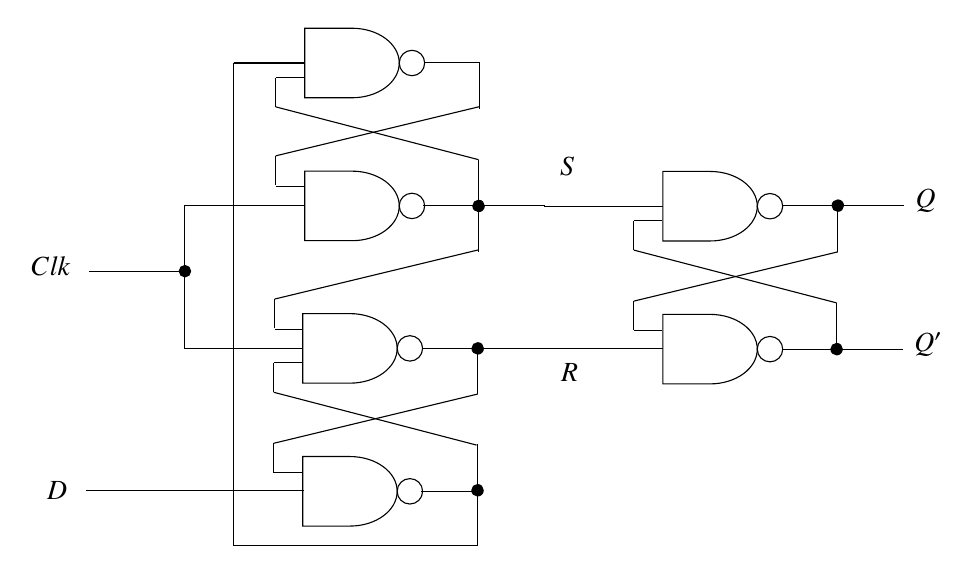
\begin{tikzpicture}[x=0.75pt,y=0.75pt,yscale=-1,xscale=1]
\draw    (337,106.71) -- (394.29,106.71) ;
\draw   (394.25,89.96) -- (417,89.96) .. controls (429.56,89.96) and (439.75,97.46) .. (439.75,106.71) .. controls (439.75,115.97) and (429.56,123.46) .. (417,123.46) -- (394.25,123.46) -- cycle ;
\draw  [fill={rgb, 255:red, 255; green, 255; blue, 255 }  ,fill opacity=1 ] (439.75,106.71) .. controls (439.75,103.33) and (442.49,100.59) .. (445.88,100.59) .. controls (449.26,100.59) and (452,103.33) .. (452,106.71) .. controls (452,110.1) and (449.26,112.84) .. (445.88,112.84) .. controls (442.49,112.84) and (439.75,110.1) .. (439.75,106.71) -- cycle ;
\draw    (452,106.43) -- (510.57,106.43) ;
\draw  [fill={rgb, 255:red, 0; green, 0; blue, 0 }  ,fill opacity=1 ] (475.8,106.43) .. controls (475.8,104.91) and (477.03,103.69) .. (478.54,103.69) .. controls (480.06,103.69) and (481.29,104.91) .. (481.29,106.43) .. controls (481.29,107.94) and (480.06,109.17) .. (478.54,109.17) .. controls (477.03,109.17) and (475.8,107.94) .. (475.8,106.43) -- cycle ;
\draw    (336.5,175.29) -- (394.29,175.29) ;
\draw   (394.25,158.82) -- (417,158.82) .. controls (429.56,158.82) and (439.75,166.32) .. (439.75,175.57) .. controls (439.75,184.82) and (429.56,192.32) .. (417,192.32) -- (394.25,192.32) -- cycle ;
\draw  [fill={rgb, 255:red, 255; green, 255; blue, 255 }  ,fill opacity=1 ] (439.75,175.57) .. controls (439.75,172.19) and (442.49,169.45) .. (445.88,169.45) .. controls (449.26,169.45) and (452,172.19) .. (452,175.57) .. controls (452,178.95) and (449.26,181.7) .. (445.88,181.7) .. controls (442.49,181.7) and (439.75,178.95) .. (439.75,175.57) -- cycle ;
\draw    (451.43,175.57) -- (510,175.57) ;
\draw  [fill={rgb, 255:red, 0; green, 0; blue, 0 }  ,fill opacity=1 ] (475.23,175.57) .. controls (475.23,174.06) and (476.46,172.83) .. (477.97,172.83) .. controls (479.49,172.83) and (480.71,174.06) .. (480.71,175.57) .. controls (480.71,177.09) and (479.49,178.31) .. (477.97,178.31) .. controls (476.46,178.31) and (475.23,177.09) .. (475.23,175.57) -- cycle ;
\draw    (478.54,109.17) -- (478.54,128.71) ;
\draw    (380.29,166.57) -- (394,166.57) ;
\draw    (380.29,152.43) -- (380.29,166.57) ;
\draw    (478.54,128.71) -- (380.29,152.43) ;
\draw    (380.29,113.71) -- (394,113.71) ;
\draw    (380.29,113.71) -- (380.29,127.86) ;
\draw    (477.97,153.29) -- (477.97,172.83) ;
\draw    (380.29,127.86) -- (477.97,153.29) ;
\draw    (163.5,175.21) -- (220.79,175.21) ;
\draw   (220.75,158.46) -- (243.5,158.46) .. controls (256.06,158.46) and (266.25,165.96) .. (266.25,175.21) .. controls (266.25,184.47) and (256.06,191.96) .. (243.5,191.96) -- (220.75,191.96) -- cycle ;
\draw  [fill={rgb, 255:red, 255; green, 255; blue, 255 }  ,fill opacity=1 ] (266.25,175.21) .. controls (266.25,171.83) and (268.99,169.09) .. (272.38,169.09) .. controls (275.76,169.09) and (278.5,171.83) .. (278.5,175.21) .. controls (278.5,178.6) and (275.76,181.34) .. (272.38,181.34) .. controls (268.99,181.34) and (266.25,178.6) .. (266.25,175.21) -- cycle ;
\draw    (278.5,175.21) -- (337.07,175.21) ;
\draw    (116.5,243.79) -- (221.29,243.79) ;
\draw   (220.75,227.32) -- (243.5,227.32) .. controls (256.06,227.32) and (266.25,234.82) .. (266.25,244.07) .. controls (266.25,253.32) and (256.06,260.82) .. (243.5,260.82) -- (220.75,260.82) -- cycle ;
\draw  [fill={rgb, 255:red, 255; green, 255; blue, 255 }  ,fill opacity=1 ] (266.25,244.07) .. controls (266.25,240.69) and (268.99,237.95) .. (272.38,237.95) .. controls (275.76,237.95) and (278.5,240.69) .. (278.5,244.07) .. controls (278.5,247.45) and (275.76,250.2) .. (272.38,250.2) .. controls (268.99,250.2) and (266.25,247.45) .. (266.25,244.07) -- cycle ;
\draw    (277.93,244.07) -- (305,244.07) ;
\draw    (206.79,235.07) -- (220.5,235.07) ;
\draw    (206.79,220.93) -- (206.79,235.07) ;
\draw    (305.04,197.21) -- (206.79,220.93) ;
\draw    (206.79,182.21) -- (220.5,182.21) ;
\draw    (206.79,182.21) -- (206.79,196.36) ;
\draw    (206.79,196.36) -- (304.47,221.79) ;
\draw  [fill={rgb, 255:red, 0; green, 0; blue, 0 }  ,fill opacity=1 ] (302.3,175.21) .. controls (302.3,173.7) and (303.53,172.47) .. (305.04,172.47) .. controls (306.56,172.47) and (307.79,173.7) .. (307.79,175.21) .. controls (307.79,176.73) and (306.56,177.96) .. (305.04,177.96) .. controls (303.53,177.96) and (302.3,176.73) .. (302.3,175.21) -- cycle ;
\draw    (305.04,177.67) -- (305.04,197.21) ;
\draw  [fill={rgb, 255:red, 0; green, 0; blue, 0 }  ,fill opacity=1 ] (302.23,243.57) .. controls (302.23,242.06) and (303.46,240.83) .. (304.97,240.83) .. controls (306.49,240.83) and (307.71,242.06) .. (307.71,243.57) .. controls (307.71,245.09) and (306.49,246.31) .. (304.97,246.31) .. controls (303.46,246.31) and (302.23,245.09) .. (302.23,243.57) -- cycle ;
\draw    (304.97,221.29) -- (304.97,240.83) ;
\draw    (187.5,37.71) -- (221.79,37.71) ;
\draw   (221.75,20.96) -- (244.5,20.96) .. controls (257.06,20.96) and (267.25,28.46) .. (267.25,37.71) .. controls (267.25,46.97) and (257.06,54.46) .. (244.5,54.46) -- (221.75,54.46) -- cycle ;
\draw  [fill={rgb, 255:red, 255; green, 255; blue, 255 }  ,fill opacity=1 ] (267.25,37.71) .. controls (267.25,34.33) and (269.99,31.59) .. (273.38,31.59) .. controls (276.76,31.59) and (279.5,34.33) .. (279.5,37.71) .. controls (279.5,41.1) and (276.76,43.84) .. (273.38,43.84) .. controls (269.99,43.84) and (267.25,41.1) .. (267.25,37.71) -- cycle ;
\draw    (279.5,37.43) -- (306.04,37.43) ;
\draw    (164,106.29) -- (221.79,106.29) ;
\draw   (221.75,89.82) -- (244.5,89.82) .. controls (257.06,89.82) and (267.25,97.32) .. (267.25,106.57) .. controls (267.25,115.82) and (257.06,123.32) .. (244.5,123.32) -- (221.75,123.32) -- cycle ;
\draw  [fill={rgb, 255:red, 255; green, 255; blue, 255 }  ,fill opacity=1 ] (267.25,106.57) .. controls (267.25,103.19) and (269.99,100.45) .. (273.38,100.45) .. controls (276.76,100.45) and (279.5,103.19) .. (279.5,106.57) .. controls (279.5,109.95) and (276.76,112.7) .. (273.38,112.7) .. controls (269.99,112.7) and (267.25,109.95) .. (267.25,106.57) -- cycle ;
\draw    (278.93,106.57) -- (337.5,106.57) ;
\draw  [fill={rgb, 255:red, 0; green, 0; blue, 0 }  ,fill opacity=1 ] (302.73,106.57) .. controls (302.73,105.06) and (303.96,103.83) .. (305.47,103.83) .. controls (306.99,103.83) and (308.21,105.06) .. (308.21,106.57) .. controls (308.21,108.09) and (306.99,109.31) .. (305.47,109.31) .. controls (303.96,109.31) and (302.73,108.09) .. (302.73,106.57) -- cycle ;
\draw    (306.04,37.43) -- (306.04,59.71) ;
\draw    (207.79,97.07) -- (221.5,97.07) ;
\draw    (207.79,82.43) -- (207.79,96.57) ;
\draw    (306.04,58.71) -- (207.79,82.43) ;
\draw    (207.79,44.71) -- (221.5,44.71) ;
\draw    (207.79,44.71) -- (207.79,58.86) ;
\draw    (305.47,84.29) -- (305.47,103.83) ;
\draw    (207.79,58.86) -- (305.47,84.29) ;
\draw    (305.54,109.17) -- (305.54,128.71) ;
\draw    (207.29,166.07) -- (221,166.07) ;
\draw    (207.29,151.43) -- (207.29,165.57) ;
\draw    (305.54,127.71) -- (207.29,151.43) ;
\draw    (187.5,37.71) -- (187.5,270.25) ;
\draw    (187.5,270.25) -- (305,270.25) ;
\draw    (304.97,246.31) -- (304.97,270.25) ;
\draw    (164,106.29) -- (164,175.21) ;
\draw  [fill={rgb, 255:red, 0; green, 0; blue, 0 }  ,fill opacity=1 ] (161.26,138.01) .. controls (161.26,136.5) and (162.49,135.27) .. (164,135.27) .. controls (165.51,135.27) and (166.74,136.5) .. (166.74,138.01) .. controls (166.74,139.52) and (165.51,140.75) .. (164,140.75) .. controls (162.49,140.75) and (161.26,139.52) .. (161.26,138.01) -- cycle ;
\draw    (118,138.01) -- (161.26,138.01) ;
\draw (514.43,97.26) node [anchor=north west][inner sep=0.75pt]    {$Q$};
\draw (513.86,166.4) node [anchor=north west][inner sep=0.75pt]    {$Q'$};
\draw (96,238) node [anchor=north west][inner sep=0.75pt]    {$D$};
\draw (88.5,129.9) node [anchor=north west][inner sep=0.75pt]    {$Clk$};
\draw (344,181.4) node [anchor=north west][inner sep=0.75pt]    {$R$};
\draw (343.5,81.9) node [anchor=north west][inner sep=0.75pt]    {$S$};
\end{tikzpicture}
\end{center}

\begin{minipage}{0.6\textwidth}
\begin{center}
\begin{table}[H]
\centering
\begin{tabular}{cc|cc}
Clk & D & Q & Q' \\ \hline
$\uparrow$ & 0 & 0 & 1 \\
$\uparrow$ & 1 & 1 & 0
\end{tabular}
\end{table}
\end{center}
\end{minipage}
\begin{minipage}{0.3\textwidth}
\begin{center}
\tikzset{every picture/.style={line width=0.75pt}}       
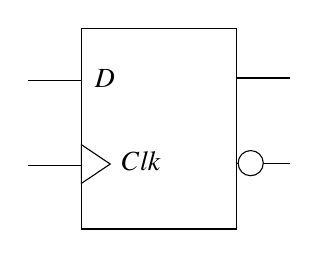
\begin{tikzpicture}[x=0.75pt,y=0.75pt,yscale=-1,xscale=1]
\draw   (167,71.5) -- (242,71.5) -- (242,168.25) -- (167,168.25) -- cycle ;
\draw   (181,136.93) -- (167.13,146.25) -- (167.13,127.62) -- cycle ;
\draw    (141.5,96.5) -- (167,96.5) ;
\draw    (141.5,137.5) -- (167,137.5) ;
\draw    (242,95.5) -- (267.5,95.5) ;
\draw    (242,136.5) -- (267.5,136.5) ;
\draw  [fill={rgb, 255:red, 255; green, 255; blue, 255 }  ,fill opacity=1 ] (242.63,136.5) .. controls (242.63,133.15) and (245.34,130.44) .. (248.69,130.44) .. controls (252.04,130.44) and (254.75,133.15) .. (254.75,136.5) .. controls (254.75,139.85) and (252.04,142.56) .. (248.69,142.56) .. controls (245.34,142.56) and (242.63,139.85) .. (242.63,136.5) -- cycle ;
\draw (172,90) node [anchor=north west][inner sep=0.75pt]    {$D$};
\draw (185,130) node [anchor=north west][inner sep=0.75pt]    {$Clk$};
\end{tikzpicture}
\end{center}
\end{minipage}

% \newpage
\paragraph{Positive-edge-triggered with Asynchronous Reset}
\begin{itemize}
    \item When $R = 0$, output $Q$ is reset to 0 regardless of $D$ or $Clk$.
    \item Value of $D$ transferred to $Q$ with every positive-edge clock signal, provided that $R = 1$.
\end{itemize}
\begin{center}
\tikzset{every picture/.style={line width=0.75pt}}       
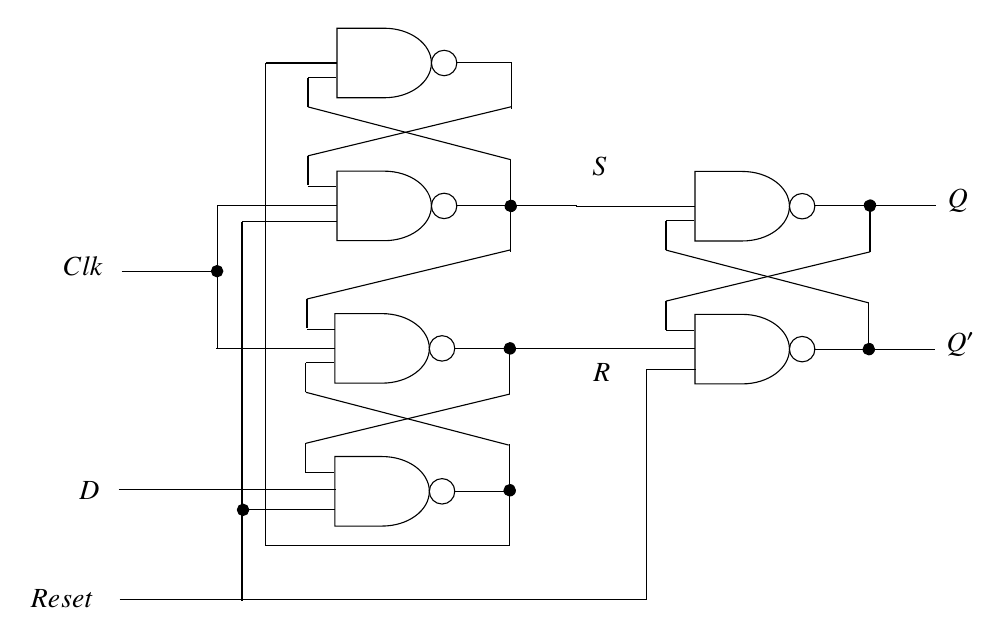
\begin{tikzpicture}[x=0.75pt,y=0.75pt,yscale=-1,xscale=1]
\draw    (337,106.71) -- (394.29,106.71) ;
\draw   (394.25,89.96) -- (417,89.96) .. controls (429.56,89.96) and (439.75,97.46) .. (439.75,106.71) .. controls (439.75,115.97) and (429.56,123.46) .. (417,123.46) -- (394.25,123.46) -- cycle ;
\draw  [fill={rgb, 255:red, 255; green, 255; blue, 255 }  ,fill opacity=1 ] (439.75,106.71) .. controls (439.75,103.33) and (442.49,100.59) .. (445.88,100.59) .. controls (449.26,100.59) and (452,103.33) .. (452,106.71) .. controls (452,110.1) and (449.26,112.84) .. (445.88,112.84) .. controls (442.49,112.84) and (439.75,110.1) .. (439.75,106.71) -- cycle ;
\draw    (452,106.43) -- (510.57,106.43) ;
\draw  [fill={rgb, 255:red, 0; green, 0; blue, 0 }  ,fill opacity=1 ] (475.8,106.43) .. controls (475.8,104.91) and (477.03,103.69) .. (478.54,103.69) .. controls (480.06,103.69) and (481.29,104.91) .. (481.29,106.43) .. controls (481.29,107.94) and (480.06,109.17) .. (478.54,109.17) .. controls (477.03,109.17) and (475.8,107.94) .. (475.8,106.43) -- cycle ;
\draw    (336.5,175.29) -- (394.29,175.29) ;
\draw   (394.25,158.82) -- (417,158.82) .. controls (429.56,158.82) and (439.75,166.32) .. (439.75,175.57) .. controls (439.75,184.82) and (429.56,192.32) .. (417,192.32) -- (394.25,192.32) -- cycle ;
\draw  [fill={rgb, 255:red, 255; green, 255; blue, 255 }  ,fill opacity=1 ] (439.75,175.57) .. controls (439.75,172.19) and (442.49,169.45) .. (445.88,169.45) .. controls (449.26,169.45) and (452,172.19) .. (452,175.57) .. controls (452,178.95) and (449.26,181.7) .. (445.88,181.7) .. controls (442.49,181.7) and (439.75,178.95) .. (439.75,175.57) -- cycle ;
\draw    (451.43,175.57) -- (510,175.57) ;
\draw  [fill={rgb, 255:red, 0; green, 0; blue, 0 }  ,fill opacity=1 ] (475.23,175.57) .. controls (475.23,174.06) and (476.46,172.83) .. (477.97,172.83) .. controls (479.49,172.83) and (480.71,174.06) .. (480.71,175.57) .. controls (480.71,177.09) and (479.49,178.31) .. (477.97,178.31) .. controls (476.46,178.31) and (475.23,177.09) .. (475.23,175.57) -- cycle ;
\draw    (478.54,109.17) -- (478.54,128.71) ;
\draw    (380.29,166.57) -- (394,166.57) ;
\draw    (380.29,152.43) -- (380.29,166.57) ;
\draw    (478.54,128.71) -- (380.29,152.43) ;
\draw    (380.29,113.71) -- (394,113.71) ;
\draw    (380.29,113.71) -- (380.29,127.86) ;
\draw    (477.97,153.29) -- (477.97,172.83) ;
\draw    (380.29,127.86) -- (477.97,153.29) ;
\draw    (163.5,175.21) -- (220.79,175.21) ;
\draw   (220.75,158.46) -- (243.5,158.46) .. controls (256.06,158.46) and (266.25,165.96) .. (266.25,175.21) .. controls (266.25,184.47) and (256.06,191.96) .. (243.5,191.96) -- (220.75,191.96) -- cycle ;
\draw  [fill={rgb, 255:red, 255; green, 255; blue, 255 }  ,fill opacity=1 ] (266.25,175.21) .. controls (266.25,171.83) and (268.99,169.09) .. (272.38,169.09) .. controls (275.76,169.09) and (278.5,171.83) .. (278.5,175.21) .. controls (278.5,178.6) and (275.76,181.34) .. (272.38,181.34) .. controls (268.99,181.34) and (266.25,178.6) .. (266.25,175.21) -- cycle ;
\draw    (278.5,175.21) -- (337.07,175.21) ;
\draw    (116.5,243.29) -- (221.29,243.29) ;
\draw   (220.75,227.32) -- (243.5,227.32) .. controls (256.06,227.32) and (266.25,234.82) .. (266.25,244.07) .. controls (266.25,253.32) and (256.06,260.82) .. (243.5,260.82) -- (220.75,260.82) -- cycle ;
\draw  [fill={rgb, 255:red, 255; green, 255; blue, 255 }  ,fill opacity=1 ] (266.25,244.07) .. controls (266.25,240.69) and (268.99,237.95) .. (272.38,237.95) .. controls (275.76,237.95) and (278.5,240.69) .. (278.5,244.07) .. controls (278.5,247.45) and (275.76,250.2) .. (272.38,250.2) .. controls (268.99,250.2) and (266.25,247.45) .. (266.25,244.07) -- cycle ;
\draw    (277.93,244.07) -- (305,244.07) ;
\draw    (206.79,235.07) -- (220.5,235.07) ;
\draw    (206.79,220.93) -- (206.79,235.07) ;
\draw    (305.04,197.21) -- (206.79,220.93) ;
\draw    (206.79,182.21) -- (220.5,182.21) ;
\draw    (206.79,182.21) -- (206.79,196.36) ;
\draw    (206.79,196.36) -- (304.47,221.79) ;
\draw  [fill={rgb, 255:red, 0; green, 0; blue, 0 }  ,fill opacity=1 ] (302.3,175.21) .. controls (302.3,173.7) and (303.53,172.47) .. (305.04,172.47) .. controls (306.56,172.47) and (307.79,173.7) .. (307.79,175.21) .. controls (307.79,176.73) and (306.56,177.96) .. (305.04,177.96) .. controls (303.53,177.96) and (302.3,176.73) .. (302.3,175.21) -- cycle ;
\draw    (305.04,177.67) -- (305.04,197.21) ;
\draw  [fill={rgb, 255:red, 0; green, 0; blue, 0 }  ,fill opacity=1 ] (302.23,243.57) .. controls (302.23,242.06) and (303.46,240.83) .. (304.97,240.83) .. controls (306.49,240.83) and (307.71,242.06) .. (307.71,243.57) .. controls (307.71,245.09) and (306.49,246.31) .. (304.97,246.31) .. controls (303.46,246.31) and (302.23,245.09) .. (302.23,243.57) -- cycle ;
\draw    (304.97,221.29) -- (304.97,240.83) ;
\draw    (187.5,37.71) -- (221.79,37.71) ;
\draw   (221.75,20.96) -- (244.5,20.96) .. controls (257.06,20.96) and (267.25,28.46) .. (267.25,37.71) .. controls (267.25,46.97) and (257.06,54.46) .. (244.5,54.46) -- (221.75,54.46) -- cycle ;
\draw  [fill={rgb, 255:red, 255; green, 255; blue, 255 }  ,fill opacity=1 ] (267.25,37.71) .. controls (267.25,34.33) and (269.99,31.59) .. (273.38,31.59) .. controls (276.76,31.59) and (279.5,34.33) .. (279.5,37.71) .. controls (279.5,41.1) and (276.76,43.84) .. (273.38,43.84) .. controls (269.99,43.84) and (267.25,41.1) .. (267.25,37.71) -- cycle ;
\draw    (279.5,37.43) -- (306.04,37.43) ;
\draw    (164,106.29) -- (221.79,106.29) ;
\draw   (221.75,89.82) -- (244.5,89.82) .. controls (257.06,89.82) and (267.25,97.32) .. (267.25,106.57) .. controls (267.25,115.82) and (257.06,123.32) .. (244.5,123.32) -- (221.75,123.32) -- cycle ;
\draw  [fill={rgb, 255:red, 255; green, 255; blue, 255 }  ,fill opacity=1 ] (267.25,106.57) .. controls (267.25,103.19) and (269.99,100.45) .. (273.38,100.45) .. controls (276.76,100.45) and (279.5,103.19) .. (279.5,106.57) .. controls (279.5,109.95) and (276.76,112.7) .. (273.38,112.7) .. controls (269.99,112.7) and (267.25,109.95) .. (267.25,106.57) -- cycle ;
\draw    (278.93,106.57) -- (337.5,106.57) ;
\draw  [fill={rgb, 255:red, 0; green, 0; blue, 0 }  ,fill opacity=1 ] (302.73,106.57) .. controls (302.73,105.06) and (303.96,103.83) .. (305.47,103.83) .. controls (306.99,103.83) and (308.21,105.06) .. (308.21,106.57) .. controls (308.21,108.09) and (306.99,109.31) .. (305.47,109.31) .. controls (303.96,109.31) and (302.73,108.09) .. (302.73,106.57) -- cycle ;
\draw    (306.04,37.43) -- (306.04,59.71) ;
\draw    (207.79,97.07) -- (221.5,97.07) ;
\draw    (207.79,82.43) -- (207.79,96.57) ;
\draw    (306.04,58.71) -- (207.79,82.43) ;
\draw    (207.79,44.71) -- (221.5,44.71) ;
\draw    (207.79,44.71) -- (207.79,58.86) ;
\draw    (305.47,84.29) -- (305.47,103.83) ;
\draw    (207.79,58.86) -- (305.47,84.29) ;
\draw    (305.54,109.17) -- (305.54,128.71) ;
\draw    (207.29,166.07) -- (221,166.07) ;
\draw    (207.29,151.43) -- (207.29,165.57) ;
\draw    (305.54,127.71) -- (207.29,151.43) ;
\draw    (187.5,37.71) -- (187.5,270.25) ;
\draw    (187.5,270.25) -- (305,270.25) ;
\draw    (304.97,246.31) -- (304.97,270.25) ;
\draw    (164,106.29) -- (164,175.21) ;
\draw  [fill={rgb, 255:red, 0; green, 0; blue, 0 }  ,fill opacity=1 ] (161.26,138.01) .. controls (161.26,136.5) and (162.49,135.27) .. (164,135.27) .. controls (165.51,135.27) and (166.74,136.5) .. (166.74,138.01) .. controls (166.74,139.52) and (165.51,140.75) .. (164,140.75) .. controls (162.49,140.75) and (161.26,139.52) .. (161.26,138.01) -- cycle ;
\draw    (118,138.01) -- (161.26,138.01) ;
\draw    (117,296.29) -- (371,296.29) ;
\draw    (371,185.25) -- (371,296.29) ;
\draw    (371,185.25) -- (394.5,185.25) ;
\draw    (176,114.25) -- (176,297) ;
\draw    (176,114.25) -- (221.75,114.25) ;
\draw    (176.5,253) -- (220.75,253) ;
\draw  [fill={rgb, 255:red, 0; green, 0; blue, 0 }  ,fill opacity=1 ] (173.76,253) .. controls (173.76,251.49) and (174.99,250.26) .. (176.5,250.26) .. controls (178.01,250.26) and (179.24,251.49) .. (179.24,253) .. controls (179.24,254.51) and (178.01,255.74) .. (176.5,255.74) .. controls (174.99,255.74) and (173.76,254.51) .. (173.76,253) -- cycle ;
\draw (514.43,97.26) node [anchor=north west][inner sep=0.75pt]    {$Q$};
\draw (513.86,166.4) node [anchor=north west][inner sep=0.75pt]    {$Q'$};
\draw (96,238) node [anchor=north west][inner sep=0.75pt]    {$D$};
\draw (88.5,129.9) node [anchor=north west][inner sep=0.75pt]    {$Clk$};
\draw (344,181.4) node [anchor=north west][inner sep=0.75pt]    {$R$};
\draw (343.5,81.9) node [anchor=north west][inner sep=0.75pt]    {$S$};
\draw (73,290) node [anchor=north west][inner sep=0.75pt]    {$Reset$};
\end{tikzpicture}
\end{center}

\begin{minipage}{0.6\textwidth}
\begin{table}[H]
\centering
\begin{tabular}{ccc|cc}
R & Clk & D & Q & Q' \\ \hline
0 & x & x & 0 & 1 \\
1 & $\uparrow$ & 0 & 0 & 1 \\
1 & $\uparrow$ & 1 & 1 & 0
\end{tabular}
\end{table}
\end{minipage}
\begin{minipage}{0.3\textwidth}
\begin{center}
\tikzset{every picture/.style={line width=0.75pt}}      
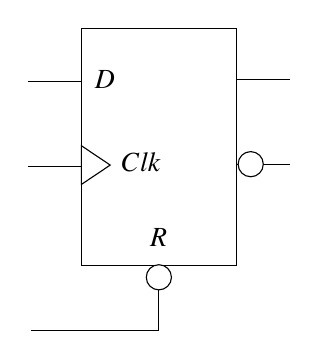
\begin{tikzpicture}[x=0.75pt,y=0.75pt,yscale=-1,xscale=1]
\draw   (167,71) -- (242,71) -- (242,185.25) -- (167,185.25) -- cycle ;
\draw   (181,136.93) -- (167.13,146.25) -- (167.13,127.62) -- cycle ;
\draw    (141.5,96.5) -- (167,96.5) ;
\draw    (141.5,137.5) -- (167,137.5) ;
\draw    (242,95.5) -- (267.5,95.5) ;
\draw    (242,136.5) -- (267.5,136.5) ;
\draw  [fill={rgb, 255:red, 255; green, 255; blue, 255 }  ,fill opacity=1 ] (242.63,136.5) .. controls (242.63,133.15) and (245.34,130.44) .. (248.69,130.44) .. controls (252.04,130.44) and (254.75,133.15) .. (254.75,136.5) .. controls (254.75,139.85) and (252.04,142.56) .. (248.69,142.56) .. controls (245.34,142.56) and (242.63,139.85) .. (242.63,136.5) -- cycle ;
\draw  [fill={rgb, 255:red, 255; green, 255; blue, 255 }  ,fill opacity=1 ] (198.38,191) .. controls (198.38,187.65) and (201.09,184.94) .. (204.44,184.94) .. controls (207.79,184.94) and (210.5,187.65) .. (210.5,191) .. controls (210.5,194.35) and (207.79,197.06) .. (204.44,197.06) .. controls (201.09,197.06) and (198.38,194.35) .. (198.38,191) -- cycle ;
\draw   (204.44,197.06) -- (204.44,216.75) -- (143,216.75) ;
\draw (172,90) node [anchor=north west][inner sep=0.75pt]    {$D$};
\draw (185,130) node [anchor=north west][inner sep=0.75pt]    {$Clk$};
\draw (199,166) node [anchor=north west][inner sep=0.75pt]    {$R$};
\end{tikzpicture}
\end{center}
\end{minipage}

\subsubsection{JK Flip-Flop}
\begin{itemize}
    \item Characteristic equation: $Q(t+1) = JQ' + K'Q$
\end{itemize}

\begin{center}
\tikzset{every picture/.style={line width=0.75pt}}
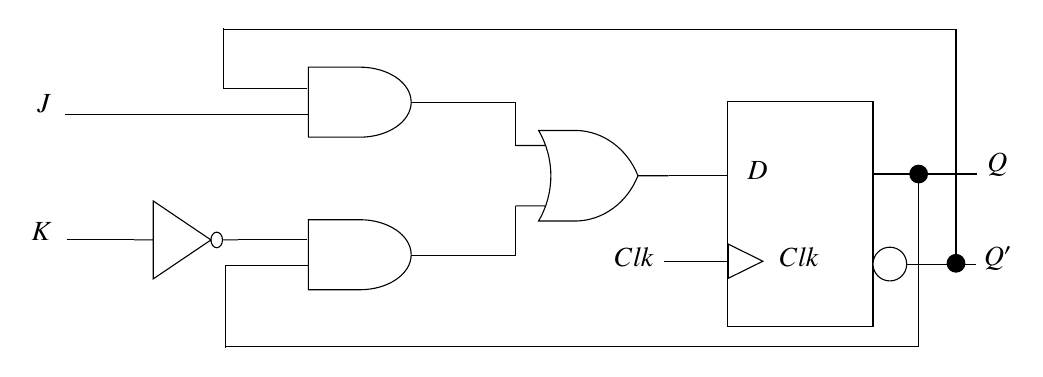
\begin{tikzpicture}[x=0.75pt,y=0.75pt,yscale=-1,xscale=1]
\draw    (491,143.88) -- (540.5,143.88) ;
\draw   (219,49) -- (243.75,49) .. controls (257.42,49) and (268.5,56.56) .. (268.5,65.88) .. controls (268.5,75.19) and (257.42,82.75) .. (243.75,82.75) -- (219,82.75) -- cycle ;
\draw   (219,122.5) -- (243.75,122.5) .. controls (257.42,122.5) and (268.5,130.06) .. (268.5,139.38) .. controls (268.5,148.69) and (257.42,156.25) .. (243.75,156.25) -- (219,156.25) -- cycle ;
\draw    (101.5,72) -- (219,72) ;
\draw   (144.26,113.5) -- (172.04,132.25) -- (144.26,151) -- (144.26,113.5) -- cycle (135,132.25) -- (144.26,132.25) (177.59,132.25) -- (185,132.25) (172.04,132.25) .. controls (172.04,130.18) and (173.28,128.5) .. (174.81,128.5) .. controls (176.35,128.5) and (177.59,130.18) .. (177.59,132.25) .. controls (177.59,134.32) and (176.35,136) .. (174.81,136) .. controls (173.28,136) and (172.04,134.32) .. (172.04,132.25) -- cycle ;
\draw    (185,132.25) -- (218.5,132.25) ;
\draw   (329.88,79.5) -- (348.3,79.5) .. controls (361.15,79.89) and (372.63,88.39) .. (377.77,101.31) .. controls (372.63,114.23) and (361.15,122.73) .. (348.3,123.13) -- (329.88,123.13) .. controls (337.78,109.63) and (337.78,93) .. (329.88,79.5) -- cycle (318.83,86.77) -- (333.57,86.77) (318.83,115.85) -- (333.57,115.85) (377.77,101.31) -- (392.5,101.31) ;
\draw   (268.5,65.88) -- (318.83,65.88) -- (318.83,86.77) ;
\draw   (268.5,139.71) -- (318.83,139.71) -- (318.83,115.85) ;
\draw    (102.5,132.25) -- (135,132.25) ;
\draw   (219.5,144.5) -- (179,144.5) -- (179,184.25) ;
\draw   (218.5,59.25) -- (178,59.25) -- (178,30.25) ;
\draw   (421,65.5) -- (491,65.5) -- (491,173.75) -- (421,173.75) -- cycle ;
\draw   (437.96,142.5) -- (421.25,150.75) -- (421.25,134.25) -- cycle ;
\draw    (390.5,142.5) -- (421,142.5) ;
\draw    (392.5,101.31) -- (421,101.31) ;
\draw  [fill={rgb, 255:red, 255; green, 255; blue, 255 }  ,fill opacity=1 ] (491,143.88) .. controls (491,139.39) and (494.64,135.75) .. (499.13,135.75) .. controls (503.61,135.75) and (507.25,139.39) .. (507.25,143.88) .. controls (507.25,148.36) and (503.61,152) .. (499.13,152) .. controls (494.64,152) and (491,148.36) .. (491,143.88) -- cycle ;
\draw    (491.5,100.5) -- (541,100.5) ;
\draw  [fill={rgb, 255:red, 0; green, 0; blue, 0 }  ,fill opacity=1 ] (508.75,100.5) .. controls (508.75,98.15) and (510.65,96.25) .. (513,96.25) .. controls (515.35,96.25) and (517.25,98.15) .. (517.25,100.5) .. controls (517.25,102.85) and (515.35,104.75) .. (513,104.75) .. controls (510.65,104.75) and (508.75,102.85) .. (508.75,100.5) -- cycle ;
\draw   (513,104.75) -- (513,183.75) -- (179.5,183.75) ;
\draw  [fill={rgb, 255:red, 0; green, 0; blue, 0 }  ,fill opacity=1 ] (526.75,143.5) .. controls (526.75,141.15) and (528.65,139.25) .. (531,139.25) .. controls (533.35,139.25) and (535.25,141.15) .. (535.25,143.5) .. controls (535.25,145.85) and (533.35,147.75) .. (531,147.75) .. controls (528.65,147.75) and (526.75,145.85) .. (526.75,143.5) -- cycle ;
\draw   (178,30.75) -- (531,30.75) -- (531,139.25) ;
\draw (86.5,61) node [anchor=north west][inner sep=0.75pt]    {$J$};
\draw (84,122.4) node [anchor=north west][inner sep=0.75pt]    {$K$};
\draw (429,93) node [anchor=north west][inner sep=0.75pt]    {$D$};
\draw (444.5,135) node [anchor=north west][inner sep=0.75pt]    {$Clk$};
\draw (365,135) node [anchor=north west][inner sep=0.75pt]    {$Clk$};
\draw (544.5,89.4) node [anchor=north west][inner sep=0.75pt]    {$Q$};
\draw (543,133.9) node [anchor=north west][inner sep=0.75pt]    {$Q'$};
\end{tikzpicture}
\end{center}

\begin{minipage}{0.6\textwidth}
\begin{table}[H]
\centering
\begin{tabular}{cc|l}
J & K & \multicolumn{1}{c}{Q(t+1)} \\ \hline
0 & 0 & Q(t)\quad No change \\
0 & 1 & 0\qquad Reset \\
1 & 0 & 1\qquad Set \\
1 & 1 & Q'(t)\quad Complement
\end{tabular}
\end{table}
\end{minipage}
\begin{minipage}{0.3\textwidth}
\begin{center}
\tikzset{every picture/.style={line width=0.75pt}}       
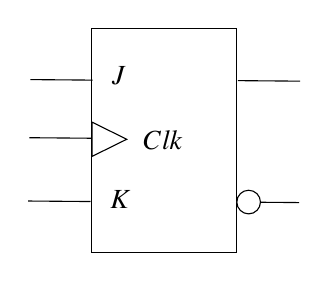
\begin{tikzpicture}[x=0.75pt,y=0.75pt,yscale=-1,xscale=1]
\draw   (246,65) -- (316,65) -- (316,173.25) -- (246,173.25) -- cycle ;
\draw   (262.96,118.5) -- (246.25,126.75) -- (246.25,110.25) -- cycle ;
\draw    (216.5,89.75) -- (246.5,90) ;
\draw    (216,117.75) -- (246,118) ;
\draw    (215.5,148.25) -- (245.5,148.5) ;
\draw    (316.5,90.25) -- (346.5,90.5) ;
\draw    (316,148.75) -- (346,149) ;
\draw  [fill={rgb, 255:red, 255; green, 255; blue, 255 }  ,fill opacity=1 ] (316,148.75) .. controls (316,145.61) and (318.55,143.06) .. (321.69,143.06) .. controls (324.83,143.06) and (327.38,145.61) .. (327.38,148.75) .. controls (327.38,151.89) and (324.83,154.44) .. (321.69,154.44) .. controls (318.55,154.44) and (316,151.89) .. (316,148.75) -- cycle ;
\draw (269.5,113) node [anchor=north west][inner sep=0.75pt]    {$Clk$};
\draw (254,82) node [anchor=north west][inner sep=0.75pt]    {$J$};
\draw (253.5,142) node [anchor=north west][inner sep=0.75pt]    {$K$};
\end{tikzpicture}
\end{center}
\end{minipage}

\subsubsection{T Flip-Flop}
\begin{itemize}
    \item Characteristic equation: $Q(t+1) = T\bigoplus Q = TQ'+T'Q$
\end{itemize}
\begin{minipage}{0.5\textwidth}
\begin{center}
\tikzset{every picture/.style={line width=0.75pt}}    
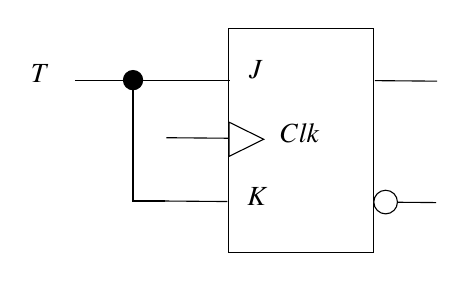
\begin{tikzpicture}[x=0.75pt,y=0.75pt,yscale=-1,xscale=1]
\draw   (246,65) -- (316,65) -- (316,173.25) -- (246,173.25) -- cycle ;
\draw   (262.96,118.5) -- (246.25,126.75) -- (246.25,110.25) -- cycle ;
\draw    (172,90) -- (246.5,90) ;
\draw    (216,117.75) -- (246,118) ;
\draw    (215.5,148.25) -- (245.5,148.5) ;
\draw    (316.5,90.25) -- (346.5,90.5) ;
\draw    (316,148.75) -- (346,149) ;
\draw  [fill={rgb, 255:red, 255; green, 255; blue, 255 }  ,fill opacity=1 ] (316,148.75) .. controls (316,145.61) and (318.55,143.06) .. (321.69,143.06) .. controls (324.83,143.06) and (327.38,145.61) .. (327.38,148.75) .. controls (327.38,151.89) and (324.83,154.44) .. (321.69,154.44) .. controls (318.55,154.44) and (316,151.89) .. (316,148.75) -- cycle ;
\draw   (200,90) -- (200,148.25) -- (215.5,148.25) ;
\draw  [fill={rgb, 255:red, 0; green, 0; blue, 0 }  ,fill opacity=1 ] (195.38,90) .. controls (195.38,87.45) and (197.45,85.38) .. (200,85.38) .. controls (202.55,85.38) and (204.63,87.45) .. (204.63,90) .. controls (204.63,92.55) and (202.55,94.63) .. (200,94.63) .. controls (197.45,94.63) and (195.38,92.55) .. (195.38,90) -- cycle ;
\draw (269.5,109.9) node [anchor=north west][inner sep=0.75pt]    {$Clk$};
\draw (254,79.4) node [anchor=north west][inner sep=0.75pt]    {$J$};
\draw (253.5,140.4) node [anchor=north west][inner sep=0.75pt]    {$K$};
\draw (149.5,81.4) node [anchor=north west][inner sep=0.75pt]    {$T$};
\end{tikzpicture}\\
Derived from $JK$ flip-flop
\end{center}
\end{minipage}
\begin{minipage}{0.5\textwidth}
\begin{center}
\tikzset{every picture/.style={line width=0.75pt}}       
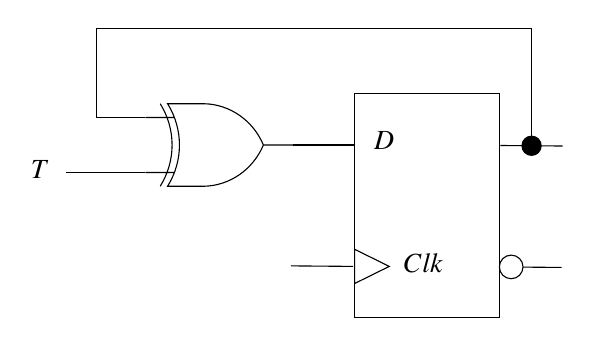
\begin{tikzpicture}[x=0.75pt,y=0.75pt,yscale=-1,xscale=1]
\draw   (246,65) -- (316,65) -- (316,173.25) -- (246,173.25) -- cycle ;
\draw   (262.96,148.5) -- (246.25,156.75) -- (246.25,140.25) -- cycle ;
\draw    (216.5,90) -- (246.5,90) ;
\draw    (215.5,148.25) -- (245.5,148.5) ;
\draw    (316.5,90.25) -- (346.5,90.5) ;
\draw    (316,148.75) -- (346,149) ;
\draw  [fill={rgb, 255:red, 255; green, 255; blue, 255 }  ,fill opacity=1 ] (316,148.75) .. controls (316,145.61) and (318.55,143.06) .. (321.69,143.06) .. controls (324.83,143.06) and (327.38,145.61) .. (327.38,148.75) .. controls (327.38,151.89) and (324.83,154.44) .. (321.69,154.44) .. controls (318.55,154.44) and (316,151.89) .. (316,148.75) -- cycle ;
\draw  [fill={rgb, 255:red, 0; green, 0; blue, 0 }  ,fill opacity=1 ] (326.88,90.38) .. controls (326.88,87.82) and (328.95,85.75) .. (331.5,85.75) .. controls (334.05,85.75) and (336.13,87.82) .. (336.13,90.38) .. controls (336.13,92.93) and (334.05,95) .. (331.5,95) .. controls (328.95,95) and (326.88,92.93) .. (326.88,90.38) -- cycle ;
\draw   (122,33.75) -- (331.5,33.75) -- (331.5,85.75) ;
\draw   (156.15,70.13) -- (173.9,70.13) .. controls (186.28,70.48) and (197.35,78.23) .. (202.3,90) .. controls (197.35,101.77) and (186.28,109.52) .. (173.9,109.88) -- (156.15,109.88) .. controls (163.76,97.58) and (163.76,82.42) .. (156.15,70.13) -- cycle (145.5,76.75) -- (159.7,76.75) (145.5,103.25) -- (159.7,103.25) (202.3,90) -- (216.5,90) (152.6,70.13) .. controls (160.21,82.42) and (160.21,97.58) .. (152.6,109.88) ;
\draw   (122,33.75) -- (122,76.75) -- (145.5,76.75) ;
\draw    (107,103.25) -- (145.5,103.25) ;
\draw (268.5,141) node [anchor=north west][inner sep=0.75pt]    {$Clk$};
\draw (254,82) node [anchor=north west][inner sep=0.75pt]    {$D$};
\draw (89,96) node [anchor=north west][inner sep=0.75pt]    {$T$};
\end{tikzpicture}\\
Derived from $D$ flip-flop
\end{center}
\end{minipage}\\[1cm]
\begin{minipage}{0.6\textwidth}
\begin{table}[H]
\centering
\begin{tabular}{c|l}
T & \multicolumn{1}{c}{Q(t+1)} \\ \hline
0 & Q(t)\quad No change \\
1 & Q'(t)\quad Reset
\end{tabular}
\end{table}
\end{minipage}
\begin{minipage}{0.3\textwidth}
\begin{center}
\tikzset{every picture/.style={line width=0.75pt}} %set default line width to 0.75pt        
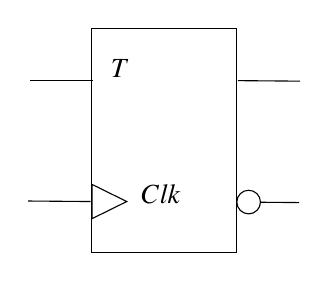
\begin{tikzpicture}[x=0.75pt,y=0.75pt,yscale=-1,xscale=1]
%uncomment if require: \path (0,300); %set diagram left start at 0, and has height of 300

%Shape: Rectangle [id:dp735450962560499] 
\draw   (246,65) -- (316,65) -- (316,173.25) -- (246,173.25) -- cycle ;
%Shape: Triangle [id:dp12373667770634089] 
\draw   (262.96,148.5) -- (246.25,156.75) -- (246.25,140.25) -- cycle ;
%Straight Lines [id:da7824632944320962] 
\draw    (216.5,90) -- (246.5,90) ;
%Straight Lines [id:da4038835614353957] 
\draw    (215.5,148.25) -- (245.5,148.5) ;
%Straight Lines [id:da5307833201587919] 
\draw    (316.5,90.25) -- (346.5,90.5) ;
%Straight Lines [id:da5339736884629156] 
\draw    (316,148.75) -- (346,149) ;
%Shape: Circle [id:dp6056445540345667] 
\draw  [fill={rgb, 255:red, 255; green, 255; blue, 255 }  ,fill opacity=1 ] (316,148.75) .. controls (316,145.61) and (318.55,143.06) .. (321.69,143.06) .. controls (324.83,143.06) and (327.38,145.61) .. (327.38,148.75) .. controls (327.38,151.89) and (324.83,154.44) .. (321.69,154.44) .. controls (318.55,154.44) and (316,151.89) .. (316,148.75) -- cycle ;

% Text Node
\draw (268.5,139.4) node [anchor=north west][inner sep=0.75pt]    {$Clk$};
% Text Node
\draw (254,78.9) node [anchor=north west][inner sep=0.75pt]    {$T$};
\end{tikzpicture}
\end{center}

\end{minipage}

\subsection{Registers}
\begin{itemize}
    \item Group of flip-flops with a common clock
    \item Each flip-flop is capable of storing 1 bit of information
\end{itemize}

\subsubsection{4-bit Register}
\begin{minipage}[t]{0.35\textwidth}
    \begin{figure}[H]
    \centering
    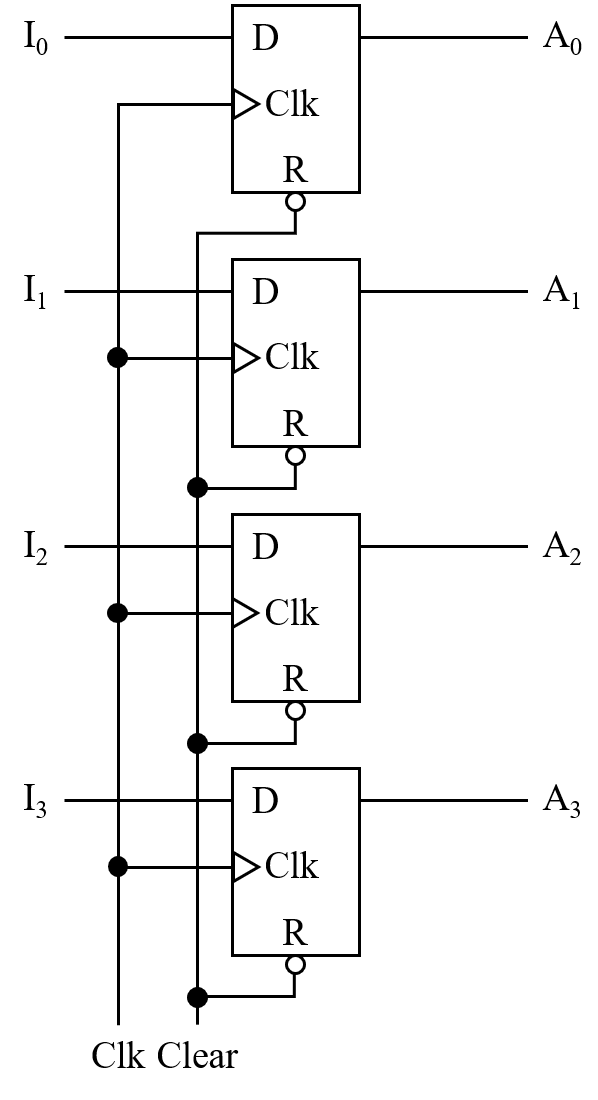
\includegraphics[width=\textwidth]{4bitreg.png}
\end{figure}
\end{minipage}
\begin{minipage}[t]{0.6\textwidth}
\begin{itemize}
    \item Triggered by positive edge of clock
    \item \texttt{Clear} must be maintained at logic 1 during clock operation
    \begin{itemize}[label=$\circ$]
        \item Allows for asynchronous reset of output values
    \end{itemize}
    \mbox{}\\
    \item Two ways for outputs to remain constant:
    \begin{enumerate}
        \item Maintain constant input values
        \item Stop the clock
    \end{enumerate}
\end{itemize}
\end{minipage}

\subsubsection{Shift Register}
\begin{itemize}
    \item Shifts binary information in each flip-flop in one direction
    \item Each clock pulse shifts value of flip-flop one position to the right
\end{itemize}
\begin{figure}[H]
    \centering
    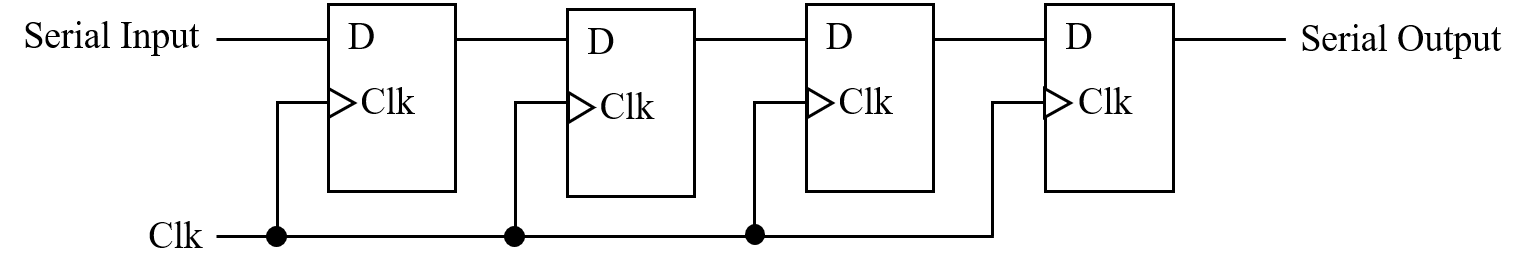
\includegraphics[width=0.8\textwidth]{serial-trf.png}
\end{figure}

\newpage
\subsubsection{Universal Shift Register}
\begin{itemize}
    \item Register that performs bidirectional bit-shift and parallel transfer operations
    \item Takes two inputs $s_0$ and $s_1$
\end{itemize}
\begin{figure}[H]
    \centering
    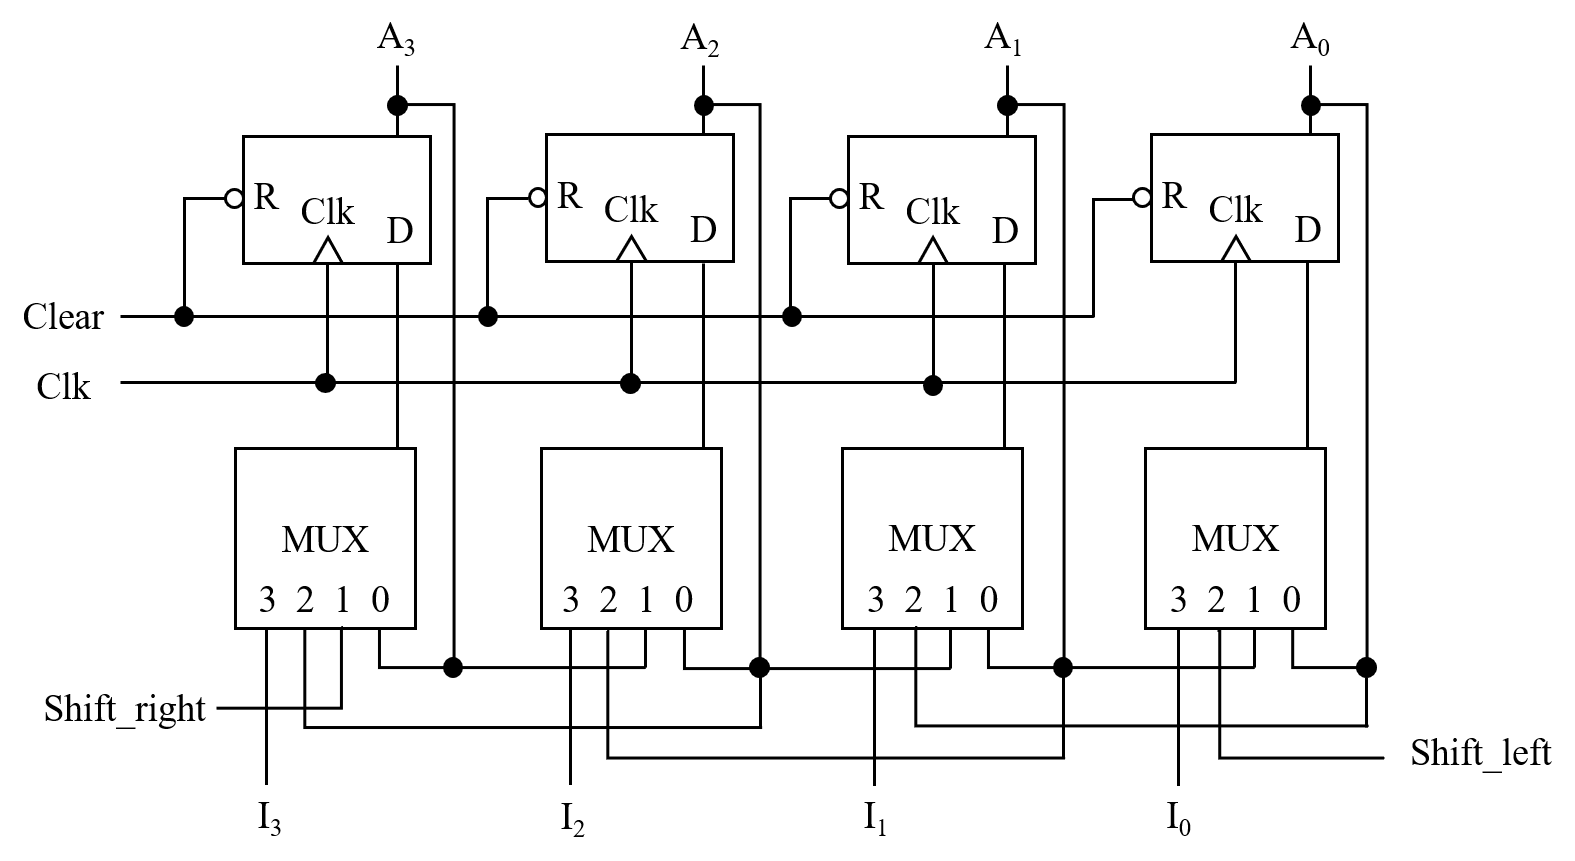
\includegraphics[width=0.85\textwidth]{uni_shift_reg.png}
\end{figure}
\begin{table}[H]
\centering
\begin{tabular}{ccc}
\multicolumn{2}{c}{\textbf{Inputs}} &  \\
$s_1$ & $s_0$ & \textbf{Register operation} \\
\hline
0 & 0 & No change \\
0 & 1 & Shift right \\
1 & 0 & Shift left \\
1 & 1 & Parallel transfer
\end{tabular}
\end{table}

\newpage
\subsection{Counters}
\begin{itemize}
    \item A register that cycles through a predetermined sequence of binary states 
\end{itemize}

\subsubsection{Binary Ripple Counter}
\begin{minipage}[t]{0.35\textwidth}
\begin{figure}[H]
    \centering
    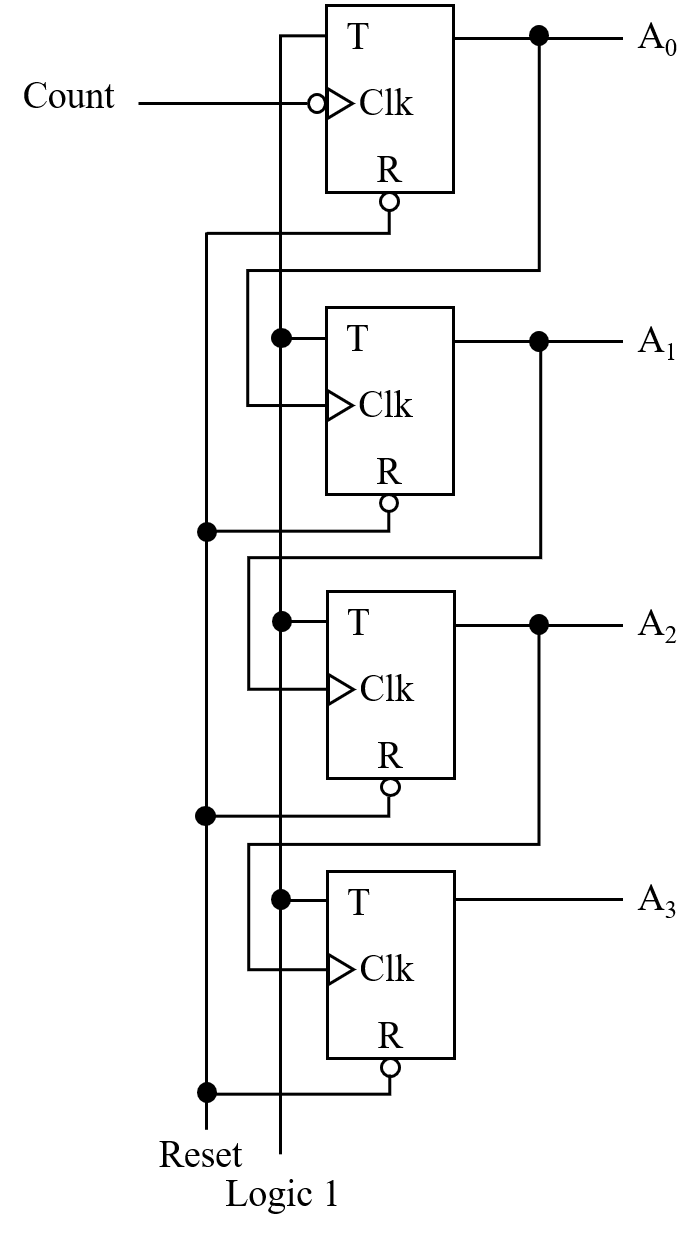
\includegraphics[width=\textwidth]{binary-ripple-counter.png}
\end{figure}
\end{minipage}
\begin{minipage}[t]{0.6\textwidth}
\begin{itemize}
    \item Negative edge triggered with asynchronous reset
    \mbox{}\\
    \item When $A_0$ goes from 1 to 0, it triggers and complements $A_1$.
    \item When $A_1$ goes from 1 to 0, it triggers and complements $A_2$.
    \item When $A_2$ goes from 1 to 0, it triggers and complements $A_3$.
\end{itemize}
\end{minipage}

\subsubsection{Binary Synchronous Counter}
\begin{minipage}[t]{0.45\textwidth}
\begin{figure}[H]
    \centering
    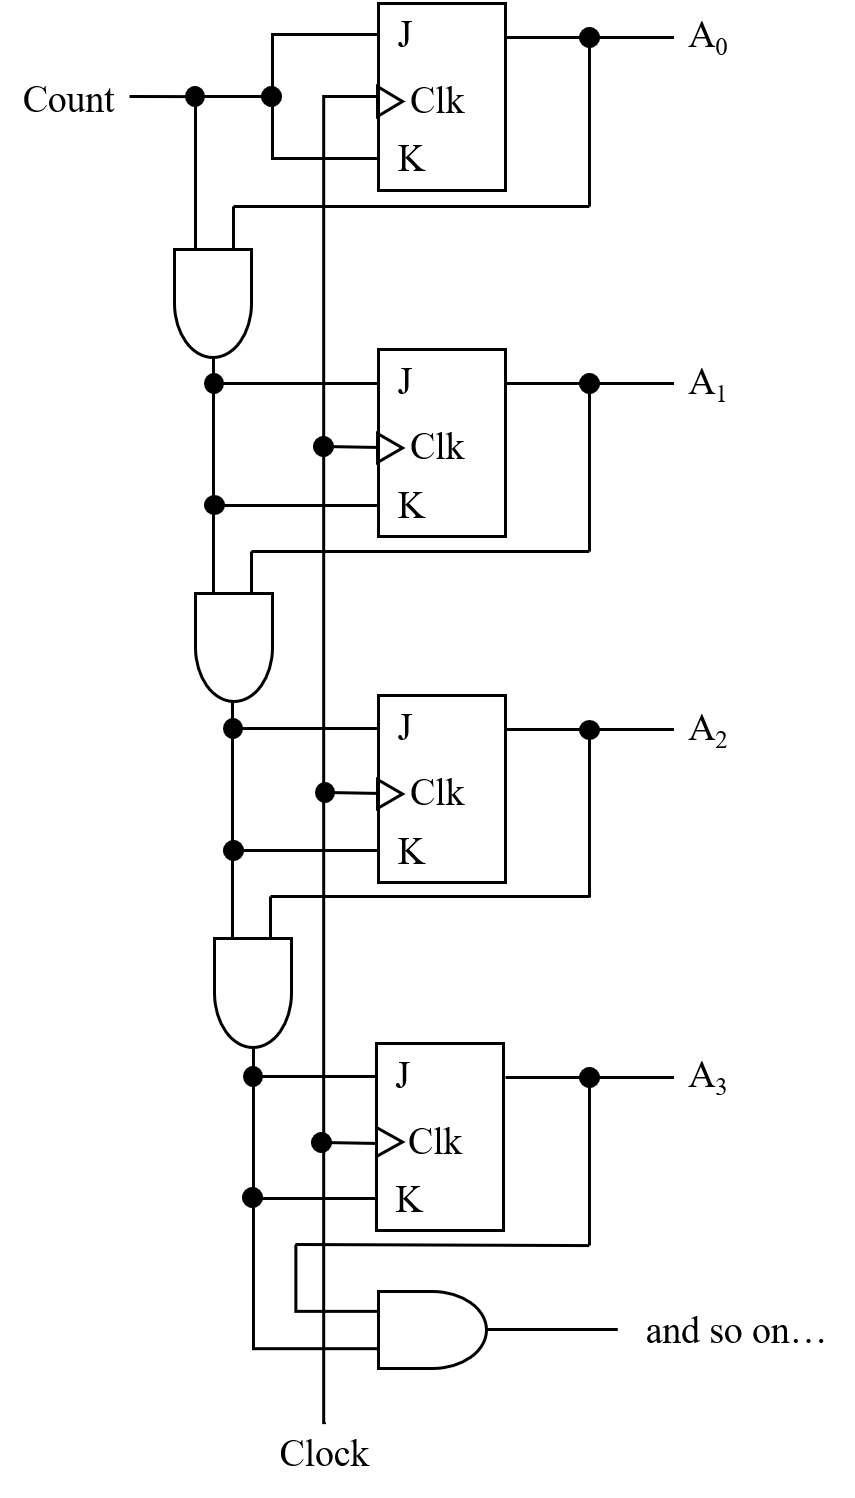
\includegraphics[width=\textwidth]{bin-sync-counter.png}
\end{figure}
\end{minipage}
\begin{minipage}[t]{0.5\textwidth}
\begin{itemize}
    \item Outputs depend on \texttt{count} and/or outputs
    \mbox{}\\
    \item When \texttt{count}$\ = 1$, $A_0$ is complemented.
    \item When \texttt{count}$\ = 1$, $A_0 = 1$, $A_1$ is complemented.
    \item When \texttt{count}$\ = 1$, $A_0 = 1$, $A_1 = 1$,\\ $A_2$ is complemented.
    \item When \texttt{count}$\ = 1$, $A_0 = 1$, $A_1 = 1$, $A_2 = 1$,\\ $A_3$ is complemented.
\end{itemize}
\end{minipage}

\newpage
\section{W5: Analysis of Sequential Circuits}

\subsection{Overview}
\begin{itemize}
    \item Analysis of sequential circuits:
    \begin{itemize}[label=$\circ$]
        \item Circuit diagram $\rightarrow$ State equation $\rightarrow$ State table $\rightarrow$ State diagram
    \end{itemize}
    \item Design of sequential circuits:
    \begin{itemize}[label=$\circ$]
        \item System specifications $\rightarrow$ State diagram $\rightarrow$ State table $\rightarrow$ Circuit/HDL
    \end{itemize}
\end{itemize}

\subsection{Analysis of Sequential Circuits}
\begin{itemize}
    \item A sequential circuit can be represented by:
    \begin{enumerate}
        \item State equations
        \item State table
        \item State diagram
    \end{enumerate}
\end{itemize}

\subsubsection{State Equation}
\begin{itemize}
    \item State equation: specifies next state as function of present state and inputs
    \begin{itemize}[label=$\circ$]
        \item Left hand side: next state of flip-flop input/output
        \item Right hand side: Boolean expression specifying present state of flip-flop inputs and inputs
    \end{itemize}
    \item Deriving state equations
    \begin{enumerate}
        \item Determine input(s), output(s) and state variables of sequential circuit.
        \begin{center}
            e.g. Input: $x$, Output: $y$, States: A, B
        \end{center}
        \item If there are JK or T flip-flops, determine flip-flop inputs in terms of present state variables and input(s).
        \begin{center}
            e.g. $\text{D}_A = Ax+Bx,\ \text{D}_B = A'x$
        \end{center}
        \item Express next state of state variables/output(s) in terms of flip-flop inputs.
        \begin{center}
            A$(t+1) = \text{D}_A = Ax+Bx,\ \text{B}(t+1) = \text{D}_B = A'x,\ y(t+1) = x'(A+B)$
        \end{center}
        \item Rewrite next state of state variables/output(s) in terms of present state variables and input(s) only.
    \end{enumerate}
\end{itemize}

\newpage
\subsubsection{State Table}
\begin{itemize}
    \item Enumerated time sequence of inputs, outputs and flip-flop states
    \item Sequential circuit with $m$ flip-flops, $n$ inputs needs $2^{m+n}$ rows in state table
\end{itemize}
\begin{table}[H]
\centering
\begin{tabular}{ccc|ccc}
\multicolumn{2}{c}{\textbf{\begin{tabular}[c]{@{}c@{}}Present \\ State\end{tabular}}} & \textbf{Input} & \multicolumn{2}{c}{\textbf{\begin{tabular}[c]{@{}c@{}}Next \\ State\end{tabular}}} & \textbf{Output} \\
A & B & $x$ & A & B & $y$ \\ \hline
0 & 0 & 0 & 0 & 0 & 0 \\
0 & 0 & 1 & 0 & 1 & 0 \\
0 & 1 & 0 & 0 & 0 & 1 \\
0 & 1 & 1 & 1 & 1 & 0 \\
1 & 0 & 0 & 0 & 0 & 1 \\
1 & 0 & 1 & 1 & 0 & 0 \\
1 & 1 & 0 & 0 & 0 & 1 \\
1 & 1 & 1 & 1 & 0 & 0
\end{tabular}\\
\mbox{}\\
e.g. A$(t+1) = \text{D}_A = Ax+Bx$\\ 
$\text{B}(t+1) = \text{D}_B = A'x$\\ 
$y(t+1) = x'(A+B)$
\end{table}

\subsubsection{State Diagram}
\begin{itemize}
    \item Graphical representation of information in state table
    \item Function of sequential circuit can be deciphered from it
\end{itemize}
\begin{minipage}{0.35\textwidth}
\begin{figure}[H]
    \centering
    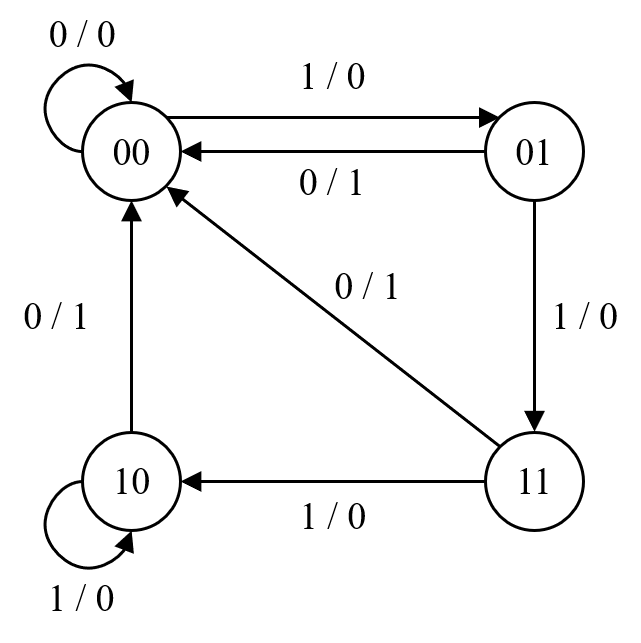
\includegraphics[width=\textwidth]{state-diagram.png}
\end{figure}
\end{minipage}
\begin{minipage}{0.5\textwidth}
\begin{center}
    e.g. Detecting a "0" in bit stream of data
\begin{itemize}
    \item Input of 0 after a series of 1's gives an output of 1
    \item State returns to initial state
\end{itemize}
\end{center}
\end{minipage}

\newpage
\subsection{Types of State Machines}

\subsubsection{Mealy Machine}
\begin{figure}[H]
    \centering
    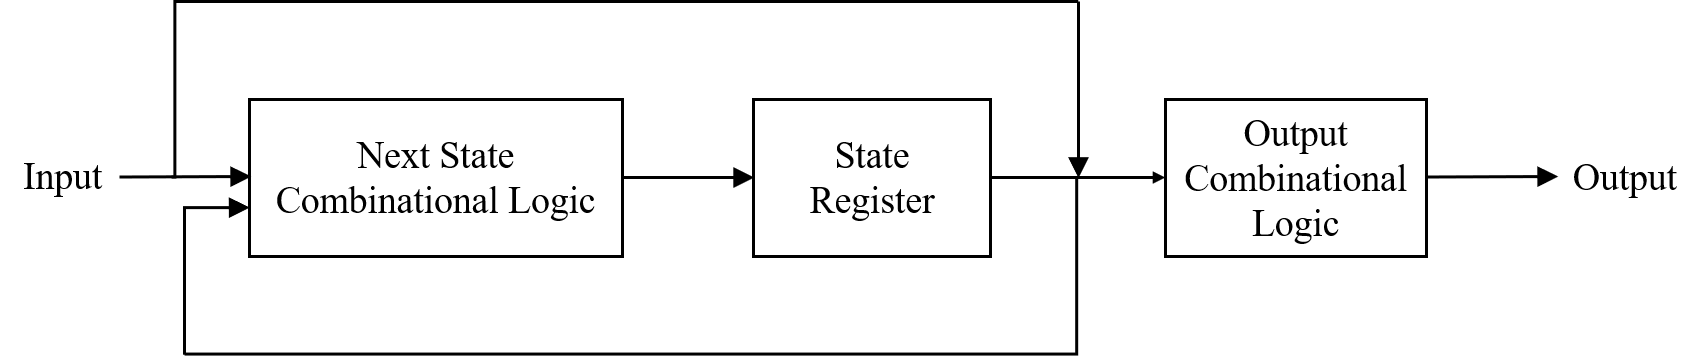
\includegraphics[width=0.85\textwidth]{mealy-machine.png}
\end{figure}
\begin{itemize}
    \item Output function of both present state and input
    \begin{itemize}[label=$\circ$]
        \item Outputs may change if inputs change during clock cycle
    \end{itemize}
    \item State symbols in state diagram: \circled{00},\ \circled{01} 
\end{itemize}

\subsubsection{Moore Machine}
\begin{figure}[H]
    \centering
    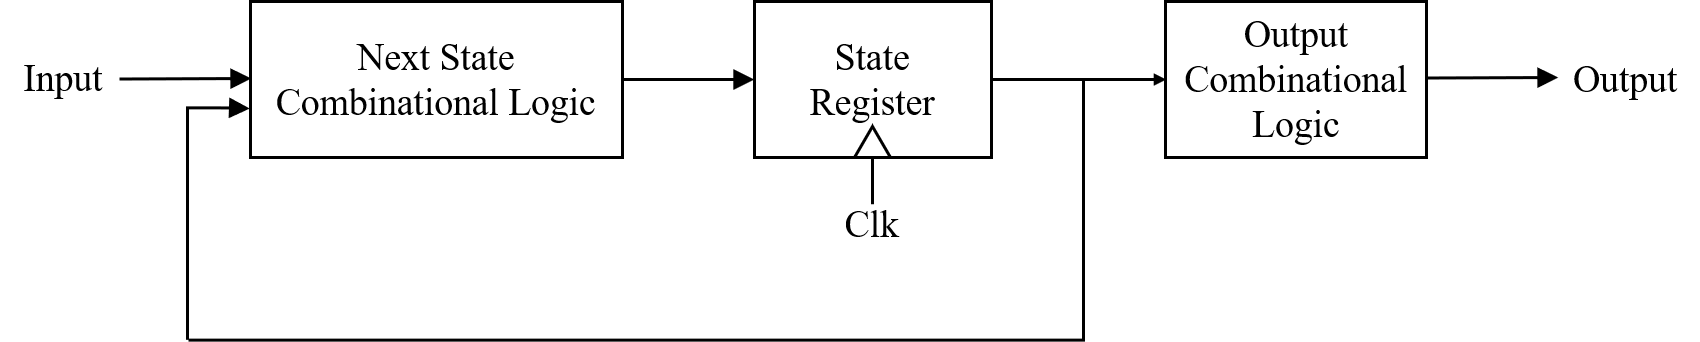
\includegraphics[width=0.85\textwidth]{moore-machine.png}
\end{figure}
\begin{itemize}
    \item Output function of only present state
    \begin{itemize}[label=$\circ$]
        \item Outputs synchronized with clock
    \end{itemize}
    \item State symbols in state diagram: \circled{00/0},\ \circled{01/1}
\end{itemize}

\subsection{State Reduction}
\begin{itemize}
    \item Reduces no. of states in state table, while keeping inputs and outputs unchanged
    \begin{itemize}[label=$\circ$]
        \item Reduces no. of flip-flops needed
    \end{itemize}
    \item Two states are equivalent if they give the same outputs and subsequent states for the same input
    \item e.g.
    \begin{minipage}{0.5\textwidth}
        \begin{table}[H]
        \centering
        \begin{tabular}{ccccc}
         & \multicolumn{2}{c}{\textbf{Next state}} & \multicolumn{2}{c}{\textbf{Output}} \\
        \textbf{Present state} & $x = 0$ & $x = 1$ & $x = 0$ & $x = 1$ \\ \hline
        e & a & f & 0 & 1 \\
        g & a & f & 0 & 1
        \end{tabular}
        \end{table}
    \end{minipage}
    \begin{minipage}{0.5\textwidth}
    \begin{itemize}[label=$\bullet$]
        \item $e$ and $g$ are equivalent states
        \item $g$ can be removed
        \item All next states to $g$ replaced with $e$
    \end{itemize}
    \end{minipage}
\end{itemize}

\newpage
\subsection{State Assignment}
\begin{itemize}
    \item Assign a unique binary value to each state
    \item e.g.
    \begin{table}[H]
    \centering
    \begin{tabular}{cccc}
    \textbf{State} & \textbf{Binary encoding} & \textbf{Gray encoding} & \textbf{One-hot encoding} \\ \hline
    a & 000 & 000 & 00001 \\
    b & 001 & 001 & 00010 \\
    c & 010 & 011 & 00100 \\
    d & 011 & 010 & 01000 \\
    e & 100 & 110 & 10000
    \end{tabular}
    \end{table}
\end{itemize}

\newpage
\section{W6: Design of Sequential Circuits}
\subsection{Overview}
\begin{itemize}
\item Design of sequential circuits:
    \begin{itemize}[label=$\circ$]
        \item System specifications $\rightarrow$ State diagram $\rightarrow$ State table $\rightarrow$ Circuit/HDL
    \end{itemize}
\end{itemize}

\subsection{Excitation Table}
\begin{itemize}
    \item Lists required inputs for a given change of state\\
    \begin{minipage}{0.5\textwidth}
    \begin{table}[H]
    \centering
    \begin{tabular}{cc|cc}
        $Q(t)$ & $Q(t+1)$ & J & K \\ \hline
        0 & 0 & 0 & x \\
        0 & 1 & 1 & x \\
        1 & 0 & x & 1 \\
        1 & 1 & x & 0
    \end{tabular}\mbox{}\\
    \mbox{}\\
    JK Flip-flop
    \end{table}
    \end{minipage}
    \begin{minipage}{0.5\textwidth}
    \begin{table}[H]
    \centering
    \begin{tabular}{cc|c}
        $Q(t)$ & $Q(t+1)$ & T \\ \hline
        0 & 0 & 0 \\
        0 & 1 & 1 \\
        1 & 0 & 1 \\
        1 & 1 & 0
    \end{tabular}\mbox{}\\
    \mbox{}\\
    T Flip-flop
    \end{table}
    \end{minipage}
    \item Derived from characteristic tables
\end{itemize}

\subsection{Steps of Sequential Logic Design}
\textbf{Designer Focus}
\begin{enumerate}
    \item Understand the problem.
    \begin{itemize}[label=$\circ$]
        \item e.g. \textit{Design a circuit that detects a sequence of three or more consecutive 1's.\\ Output 1 after three or more consecutive 1's, 0 otherwise.}
    \end{itemize}
    \item Obtain abstract representation of finite state machine e.g. state diagram.
    \begin{figure}[H]
    \centering
    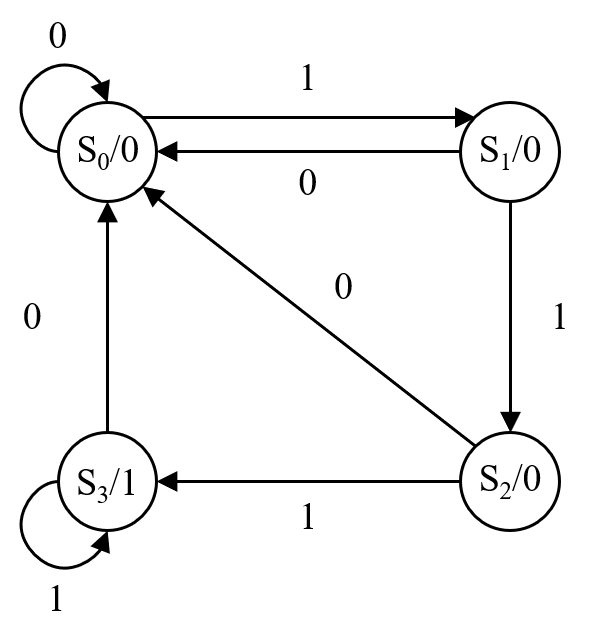
\includegraphics[width=0.35\textwidth]{seq-logic-2.png}
\end{figure}
    \item Perform state assignment.
    \begin{table}[H]
    \centering
    \begin{tabular}{cc}
        \textbf{State} & \textbf{Binary value} \\ \hline
        $S_0$ & 00 \\
        $S_1$ & 01 \\
        $S_2$ & 10 \\
        $S_3$ & 11
    \end{tabular}
    \end{table}
\end{enumerate}
\textbf{Performed by Synthesis Tool}
\begin{enumerate}[resume]
    \item Obtain state table.
    \begin{table}[H]
    \centering
    \begin{tabular}{ccc|ccc|cccc}
        \multicolumn{2}{c}{\textbf{Present state}} & \textbf{Input} & \multicolumn{2}{c}{\textbf{Next state}} & \textbf{Output} & \multicolumn{4}{c}{\textbf{Flip-flop inputs}} \\
        A & B & $x$ & A & B & $y$ & $J_A$ & $J_B$ & $K_A$ & $K_B$ \\ \hline
        0 & 0 & 0 & 0 & 0 & 0 & 0 & x & 0 & x \\
        0 & 0 & 1 & 0 & 1 & 0 & 0 & x & 1 & x \\
        0 & 1 & 0 & 1 & 0 & 0 & 1 & x & x & 1 \\
        0 & 1 & 1 & 0 & 1 & 0 & 0 & x & x & 0 \\
        1 & 0 & 0 & 0 & 0 & 0 & x & 0 & 0 & x \\
        1 & 0 & 1 & 1 & 1 & 0 & x & 0 & 1 & x \\
        1 & 1 & 0 & 0 & 0 & 1 & x & 0 & x & 0 \\
        1 & 1 & 1 & 1 & 1 & 1 & x & 1 & x & 1
    \end{tabular}
    \end{table}
    \item Perform state minimization.
    \begin{figure}[H]
    \centering
    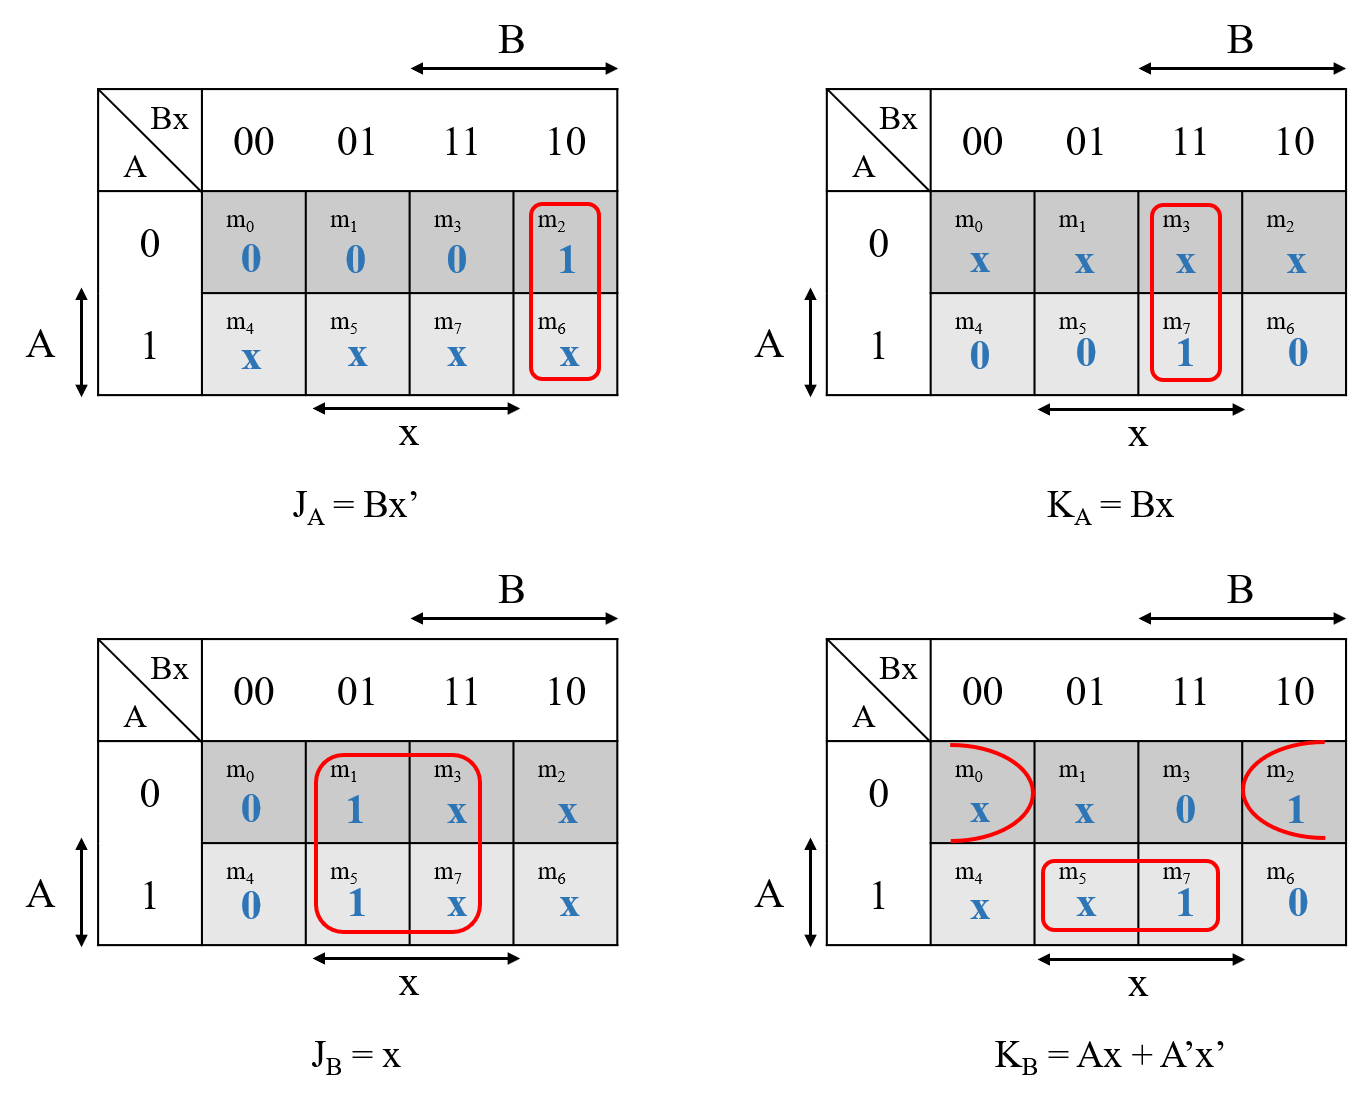
\includegraphics[width=0.8\textwidth]{state-minimization.png}
    \end{figure}
    \newpage
    \item Implement finite state machine.
    \begin{figure}[H]
    \centering
    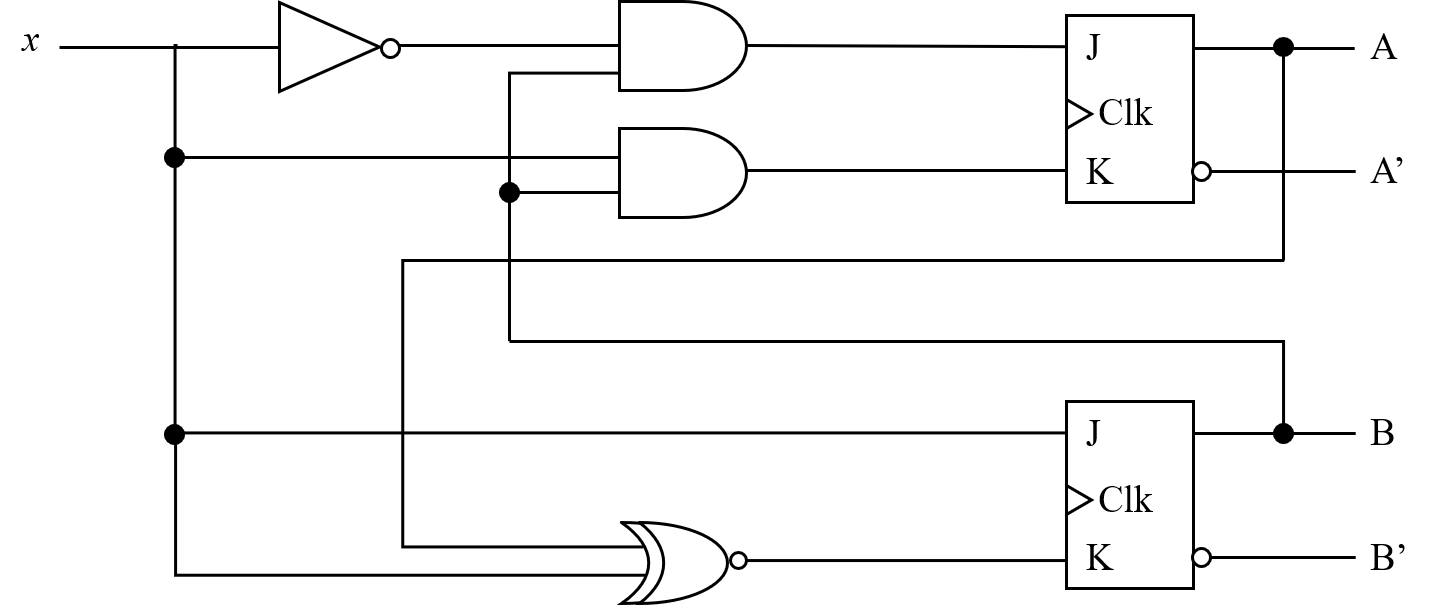
\includegraphics[width=0.8\textwidth]{seq-fsm.png}
    \end{figure}
\end{enumerate}

\newpage
\section{Miscellaneous Definitions}
\subsection{Comparison between Tables}
\begin{itemize}
    \item A \textbf{truth table} describes a combinational circuit.
    \item A \textbf{state table} describes a sequential circuit.
    \item A \textbf{characteristic table} describes the operation of a flip-flop.
    \item A \textbf{excitation table} gives the values of flip-flop inputs for a given state transition.
\end{itemize}

\subsection{Comparison between Equations}
\begin{itemize}
    \item A \textbf{Boolean equation} is an algebraic expression of a truth table.
    \item A \textbf{state equation} is an algebraic expression of a state table.
    \item A \textbf{characteristic equation} is an algebraic expression of a characteristic table.
    \item A \textbf{flip-flop input equation} is an algebraic expression of an excitation table.
\end{itemize}
\end{document}